% !TEX root = ../OT4ML.tex

\chapter{Generalized OT Problems}
\label{sec-generalized-ot-problems}

This chapter changes the optimization problem rather than only the ground distance. Barycenters average several measures, multi-marginal OT couples many measures at once, low-rank and capacity constraints restrict the admissible plans, inverse OT learns the cost from observed transport, and weak or martingale OT acts on conditional laws. These models remain close to Kantorovich optimization, but the unknown can now be a family of couplings, a factored plan, a learned cost, or a coupling subject to nonlinear conditional constraints.
\index{linear!programming}% strictindex
\index{multi-marginal!OT}% strictindex
\index{barycenter}% strictindex

\section{OT Barycenters}
\index{Wasserstein!barycenter}% strictindex
\label{sec-barycenters}

Barycenters ask how to average probability measures rather than points. This section explains the variational definition, the special closed forms in one dimension and for Gaussians, and the entropic algorithms used in practice.
\index{probability measure}% strictindex

\paragraph{Fr\'echet means.}
\index{Frechet mean}% strictindex

The natural formulation is a Fr\'echet-mean problem on the space of probability measures: the unknown is the barycenter measure itself, and its support is not prescribed. Given input measures $(\be_s)_{s=1}^S$ on a space $\Xx$ and weights $\la\in\simplex_S$, discard any zero-weight inputs and consider
\index{Wasserstein!barycenter}% strictindex
\eql{\label{eq-barycenter-generic}
	\umin{\al \in \Mm_+^1(\Xx)} \sum_{s=1}^S \la_s \MK_{\c}(\al,\be_s).
}
Any minimizer is a barycenter. Unlike a coupling, it is a new probability measure on $\Xx$.
\index{probability measure}% strictindex

This barycenter problem was introduced by Agueh and Carlier~\cite{Carlier_wasserstein_barycenter}, following earlier ideas of Carlier and Ekeland~\cite{carlierekelandmatching}. For the quadratic cost on $\Xx=\RR^d$, a barycenter exists under the usual finite-second-moment assumption. It is unique if at least one positive-weight input is absolutely continuous; more general uniqueness criteria replace absolute continuity by conditions ensuring an essentially unique multi-marginal barycentric map. Discrete existence, consistency and fixed-point constructions are further studied in~\cite{anderes2016discrete,alvarez2016fixed,leGouic2016existence}.
\index{quadratic!cost}% strictindex
\index{barycenter}% strictindex

\paragraph{Fixed-support restriction.}
\index{barycenter!fixed support}% strictindex
For computation, one often turns the preceding infinite-dimensional problem into a finite one by prescribing possible barycenter locations. Assume the inputs are discrete,
\[
	\be_s=\sum_{j=1}^{n_s} b_{s,j}\de_{x_{s,j}},
	\qquad \b_s=(b_{s,j})_{j=1}^{n_s}\in\simplex_{n_s}.
\]
Choose candidate barycenter sites $(y_i)_{i=1}^n$ and restrict the unknown to $\al=\sum_i a_i\de_{y_i}$. For each input $s$, the cost $\MK_\c(\al,\be_s)$ then becomes a finite Kantorovich problem with cost matrix
\[
	(\C_s)_{ij}=c(y_i,x_{s,j}) \in \RR^{n\times n_s}.
\]
The resulting fixed-support discrete barycenter problem is
\index{multi-marginal!OT}% strictindex
\index{discrete!barycenter}% strictindex
\index{barycenter!support}% strictindex
\eql{\label{eq-wass-discr}
	\umin{\a \in \simplex_n} \sum_{s=1}^S \la_s \MKD_{\C_s}(\a,\b_s),
}
where $\a=(a_i)_i$ are the weights on the prescribed barycenter support.
\index{histogram}% strictindex
\index{cost!matrix}% strictindex

This construction is a finite-dimensional restriction, not an exact discrete reduction of the general barycenter problem. In the ordinary two-marginal Kantorovich problem, once both marginals are discrete, the two supports are known and the whole problem is exactly a matrix optimization on their product support. For barycenters, the input supports do not determine the support of the unknown barycenter: a minimizer may place mass outside the chosen sites $(y_i)_i$ and outside the union of the input supports.

For quadratic costs, the multi-marginal formulation of Section~\ref{sec-multimarginal-ot} shows that, for discrete inputs, one may choose a barycenter supported on weighted averages $\sum_s\la_s x_{s,i_s}$ of one support point from each input. This exact candidate set can contain $\prod_s n_s$ points, which is usually too large. Prescribing the support $(y_i)_i$ before solving~\eqref{eq-wass-discr} is therefore a numerical approximation, and choosing this support is itself a significant part of the barycenter problem.
\index{multi-marginal!OT}% strictindex

\begin{example}[Application to fair score repair]\label{ex-fair-score-repair}
\index{fairness}% strictindex
\index{Wasserstein!barycenter}% strictindex
	Let \(S\) be a protected group and \(Y=f(X)\) a score. A basic demographic-parity constraint asks that the conditional laws \(\al_s=\mathcal L(Y\mid S=s)\) be independent of \(s\). OT post-processing chooses a common fair law, often a Wasserstein barycenter
	\[
		\bar\al\in\uargmin{\zeta}\sum_s p_s\Wass_2^2(\al_s,\zeta),
	\]
	and transports each group toward it. In one dimension this uses monotone rearrangements; in the quadratic absolutely continuous case it uses Brenier maps \((T_s)_\sharp\al_s=\bar\al\); otherwise one can use the barycentric projection of an optimal plan. The repaired score is \(\widetilde Y=T_S(Y)\) when a map is used. The barycenter is the compromise distribution, while the OT maps give minimal geometric changes to the original scores~\cite{DelBarrioGamboaGordalizaLoubes2018FairOT,ChzhenDenisHebiriOnetoPontil2020FairBarycenters,BuylDeBie2022FairClassifiers,HuRatzCharpentier2023FairBarycenters}. Thus the barycenter is not only an averaging tool: it can define a target distribution used to repair several observed laws simultaneously.
\end{example}


\begin{example}[Two measures recover a Wasserstein geodesic]
\index{Wasserstein!geodesic}% strictindex
	For $S=2$, $c(x,y)=\norm{x-y}^2$ and weights $(1-t,t)$, the barycenter is the point at time $t$ on a Wasserstein geodesic between $\beta_0$ and $\beta_1$. If $T$ is the Brenier map from $\beta_0$ to $\beta_1$, this barycenter is $((1-t)\Id+tT)_\sharp\beta_0$, the McCann interpolation of Definition~\ref{def-monge-mccann-interpolation}. If no Monge map is available, Definition~\ref{def-w2-geodesic-induced-by-plan} uses an optimal coupling $\pi$ and gives the barycenter as the push-forward of $\pi$ by $(x,y)\mapsto(1-t)x+ty$.
\index{Monge!problem}% strictindex
\index{optimal coupling}% strictindex
\index{McCann!interpolation}% strictindex
\index{convexity!geodesic}% strictindex
\index{interpolation map}% strictindex
\index{Brenier!map}% strictindex
\end{example}
\begin{example}[Dirac inputs recover Fr\'echet means]
	The general barycenter formulation above extends the computation of barycenters of points $(x_s)_{s=1}^S \in \Xx^S$ to arbitrary measures. Indeed, if $\be_s=\de_{x_s}$ is a single Dirac mass, then a solution is $\de_{x^\star}$, where $x^\star$ minimizes $x\mapsto\sum_s\lambda_s c(x,x_s)$.
\index{Frechet mean}% strictindex
\index{Dirac mass}% strictindex
\end{example}

\begin{figure}[ht]
\centering
\begin{tabular}{@{}cc@{}}
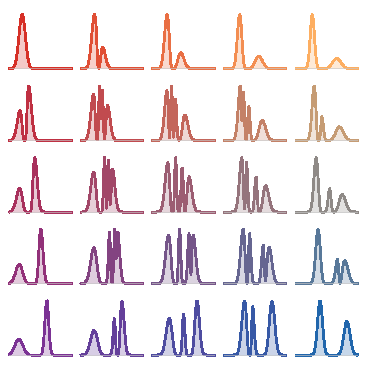
\includegraphics[width=.42\linewidth]{figures/barycenters-four-shapes/quantile-grid.pdf} &
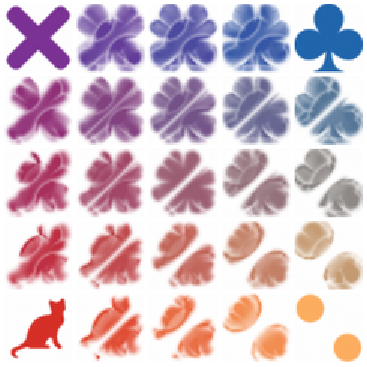
\includegraphics[width=.42\linewidth]{figures/barycenters-four-shapes/shape-grid.pdf}
\\[-.1em]
\small one-dimensional quantile barycenters &
\index{quantile!barycenter}% strictindex
\small two-dimensional entropic barycenters
\index{entropic!barycenter}% strictindex
\end{tabular}
\caption{\emph{Wasserstein barycenter grids for four corner measures.} The left panel uses the one-dimensional formula $Q_{u,v}=\sum_{i,j}\lambda_{ij}(u,v)Q_{ij}$ for one Gaussian law and three asymmetric two-Gaussian mixtures, and displays densities reconstructed from the averaged quantiles. The right panel computes entropic Wasserstein barycenters on a common pixel grid for the cat, two-disk, cross and clover silhouettes, using the normalized squared ground cost, $\epsilon=4\cdot10^{-4}$ and a Sinkhorn tolerance of $5\cdot10^{-8}$. The barycenters are rendered as density images with values clamped at their $95\%$ quantile rather than by threshold contours. Colors interpolate between the four corners and encode the same bilinear weights in both panels.}
\index{Gaussian!mixture}% strictindex
\index{Wasserstein!barycenter}% strictindex
\label{fig:barycenters-four-shapes}
\end{figure}

\begin{rem}[Mean of a quadratic barycenter]
\index{quadratic!barycenter}% strictindex
\index{barycenter!mean}% strictindex
	For $c(x,y)=\norm{x-y}^2$, the mean of the barycenter $\al^\star$ is necessarily the barycenter of the means,
	\eq{
			\int_\Xx x \d\al^\star(x) = \sum_s \la_s \int_\Xx x \d\be_s(x).
	}
	To see this, write $m_\alpha=\int x\d\alpha(x)$ and let $\alpha^0=(x\mapsto x-m_\alpha)_\sharp\alpha$ be the centered translate. Then
	\[
		\Wass_2^2(\alpha,\beta)
		=
		\norm{m_\alpha-m_\beta}^2+\Wass_2^2(\alpha^0,\beta^0).
	\]
	Indeed, the cross term vanishes under every coupling of the centered measures. The barycenter objective therefore separates into a centered term and the strictly convex Euclidean function $m\mapsto\sum_s\lambda_s\norm{m-m_{\beta_s}}^2$, whose minimizer is $\sum_s\lambda_s m_{\beta_s}$. If the input measures have compact support, the multi-marginal construction of Proposition~\ref{prop-multimarginal-barycenter} also gives a barycenter supported in the convex hull of the input supports.
\index{Wasserstein!distance}% strictindex
\index{multi-marginal!OT}% strictindex
\end{rem}

The next elementary proposition explains why the general barycenter formulation is a convex optimization problem over measures. The difficulty is not convexity, but the fact that the unknown is itself a measure whose support is not known in advance.

\begin{prop}[Convexity of the OT cost]\label{prop-barycenter-ot-cost-convexity}
\index{cost!transport}% strictindex
	The extended-valued map $(\al,\be)\mapsto\MK_\c(\al,\be)$ is jointly convex on pairs of probability measures.
\end{prop}

\begin{proof}
	Let $(\al_0,\be_0)$ and $(\al_1,\be_1)$ be two pairs of probability measures and let $t\in[0,1]$. The endpoint cases $t\in\{0,1\}$ are identities. Assume therefore that $t\in(0,1)$. If either value on the right-hand side of the convexity inequality is infinite, the claim is immediate. Otherwise, for $\eta>0$, choose couplings $\pi_i\in\Couplings(\al_i,\be_i)$ such that
\index{probability measure}% strictindex
	\[
		\int c\d\pi_i\leq\MK_\c(\al_i,\be_i)+\eta
		\qquad (i=0,1).
	\]
	Then $\pi_t=(1-t)\pi_0+t\pi_1$ is a coupling between $(1-t)\al_0+t\al_1$ and $(1-t)\be_0+t\be_1$. Hence
	\[
		\MK_\c((1-t)\al_0+t\al_1,(1-t)\be_0+t\be_1)
		\leq
		(1-t)\MK_\c(\al_0,\be_0)+t\MK_\c(\al_1,\be_1)+\eta.
	\]
	Letting $\eta\to0$ gives the claim.
\end{proof}

%%%%%%%%%%%%%%%%%%%%%%%%%%%%%%%%%%%%%%%%%%%%%%%%%%%%%%%%%%%%%%%%%%%%%%%%%%%
\paragraph{One-dimensional case.}

On the line, barycenters become linear after the quantile change of variables. This gives the rare case where the barycenter is explicit rather than the solution of a high-dimensional optimization problem.
\index{change of variables formula}% strictindex

\begin{prop}[Quantile barycenters on the line]\label{prop-quantile-barycenters}
\index{quantile!barycenter}% strictindex
	For $\Xx=\RR$ and $c(x,y)=|x-y|^2$, the quantile function of a Wasserstein barycenter is the weighted average of the input quantile functions:
\index{Wasserstein!barycenter}% strictindex
\index{quantile!function}% strictindex
	\[
		\cumul{\al^\star}^{-1}(r)
		=
		\sum_{s=1}^S\la_s\cumul{\be_s}^{-1}(r),
		\qquad r\in(0,1).
	\]
\end{prop}

\begin{proof}
	The one-dimensional formula~\eqref{eq-wass-cumul} gives
	\[
		\sum_s\la_s\Wass_2^2(\al,\be_s)
		=
		\int_0^1
		\sum_s\la_s
		\abs{\cumul{\al}^{-1}(r)-\cumul{\be_s}^{-1}(r)}^2
		\d r.
	\]
	The minimization decouples pointwise in $r$. For each fixed $r$, the minimizer of $z\mapsto\sum_s\la_s|z-\cumul{\be_s}^{-1}(r)|^2$ is the weighted average $\sum_s\la_s\cumul{\be_s}^{-1}(r)$. This function is nondecreasing because it is a positive weighted sum of nondecreasing quantile functions, hence it is a valid quantile function.
\index{quantile!function}% strictindex
\end{proof}


%%%%%%%%%%%%%%%%%%%%%%%%%%%%%%%%%%%%%%%%%%%%%%%%%%%%%%%%%%%%%%%%%%%%%%%%%%%
\paragraph{Sliced and Radon barycenters.}
\index{sliced barycenter}% strictindex
\index{Radon barycenter}% strictindex
\index{Radon sinogram}% strictindex
\index{sliced Wasserstein!barycenter}% strictindex
\index{Radon Wasserstein barycenter}% strictindex
\index{Radon transform}% strictindex

Slicing gives a scalable surrogate for high-dimensional barycenters by applying the preceding one-dimensional quantile formula in every projection direction. For measures on $\RR^d$, define the sliced barycenter by replacing $\Wass_2$ with $\SW_2$, introduced in Definition~\ref{def-sliced-wasserstein} and interpreted through the Radon transform in Section~\ref{sec-sliced-wasserstein}:
\[
	\umin{\al\in\Mm_+^1(\RR^d)}
	\sum_{s=1}^S\la_s\SW_2(\al,\be_s)^2
	=
	\umin{\al\in\Mm_+^1(\RR^d)}
	\int_{\Sphere^{d-1}}
	\sum_{s=1}^S\la_s
	\Wass_2\big((P_\theta)_\sharp\al,(P_\theta)_\sharp\be_s\big)^2
	\d\sigma(\theta).
\]
The constraint that all projected measures come from the same $\al$ is the nontrivial part of this problem. A cheaper Radon-domain approximation drops this consistency constraint and minimizes directly over collections $(\gamma_\theta)_{\theta\in\Sphere^{d-1}}$ of one-dimensional probability measures,
\[
	\umin{(\gamma_\theta)_\theta}
	\int_{\Sphere^{d-1}}
	\sum_{s=1}^S\la_s
	\Wass_2(\gamma_\theta,\be_{s,\theta})^2
	\d\sigma(\theta),
	\qquad
	\be_{s,\theta}\eqdef(P_\theta)_\sharp\be_s.
\]
This problem decouples over directions. For each $\theta$, the minimizer is the one-dimensional barycenter $\gamma_\theta$ with quantile
\[
	\cumul{\gamma_\theta}^{-1}(r)
	=
	\sum_{s=1}^S\la_s\cumul{\be_{s,\theta}}^{-1}(r),
	\qquad r\in[0,1].
\]
This relaxed value is a lower bound on the sliced barycenter value. If the minimizing family is Radon-consistent, meaning that there exists a probability measure $\bar\al$ on $\RR^d$ such that $\gamma_\theta=(P_\theta)_\sharp\bar\al$ for $\sigma$-almost every $\theta$, then this lower bound is attained and $\bar\al$ is an exact sliced barycenter.

In numerical imaging, one commonly reconstructs an approximate display density by filtered back-projection. Writing $h(\theta,t)$ for a density of $\gamma_\theta$ and $\widehat h(\theta,\omega)$ for the one-dimensional Fourier transform in $t$, the formal pseudo-inverse is
\[
	R^\dagger h(x)
	=
	c_d\int_{\Sphere^{d-1}}\int_{\RR}
	e^{\imath\omega\dotp{\theta}{x}}
	|\omega|^{d-1}
	\widehat h(\theta,\omega)
	\d\omega\,\d\sigma(\theta),
\]
\index{tomography}% strictindex
\index{ramp filter}% strictindex
\index{Radon pseudo-inverse}% strictindex
with a constant $c_d$ depending only on the Fourier convention and on the normalization of $\sigma$. This is the filtered back-projection formula used in tomography~\cite{HermanTomography}, with the multiplier $|\omega|^{d-1}$ as the ramp filter. In practice one regularizes the ramp filter and projects the reconstruction back to nonnegative densities, since low-amplitude streaks are a numerical artifact of inverting incomplete or slightly inconsistent Radon data. The construction is fast and was introduced for sliced and Radon Wasserstein barycenters in~\cite{2013-Bonneel-barycenter}, but it should not be confused with the exact variational sliced barycenter. In the continuous all-directions setting, the Radon transform is injective by the Cram\'er--Wold theorem; the issue is instead that independently averaged one-dimensional barycenters need not satisfy the range conditions of a genuine Radon transform, such as antipodal symmetry and moment consistency. With finitely many directions, the sampled Radon operator is also non-injective, so the pseudo-inverse reconstruction and the constrained sliced barycenter may differ.
\index{filtered back-projection}% strictindex
\index{Radon range condition}% strictindex
\index{Fourier transform}% strictindex
\index{Cramer-Wold theorem}% strictindex

\begin{figure}[H]
\centering

\includegraphics[width=.98\linewidth]{figures/sliced-radon-barycenter/grid.pdf}
\caption{\emph{Radon-domain sliced barycentric interpolation between the cat and heart densities.} The columns correspond to $t=0,0.2,\ldots,1$. The first row shows the endpoint densities and the intermediate regularized filtered-back-projection reconstructions $A_t$, with low-amplitude inversion ghosts suppressed in the display. The second row shows the corresponding Radon sinograms $R_t$, obtained for intermediate times by converting the directionwise quantile barycenters back into one-dimensional projected densities. The third row shows the quantile fields $Q_t(\theta,r)=(1-t)Q_0(\theta,r)+tQ_1(\theta,r)$ in Radon space. This illustrates both the simplicity of one-dimensional quantile interpolation and the extra pseudo-inverse reconstruction step needed to return from Radon data to an image density.}
\label{fig:sliced-radon-barycenter}
\end{figure}


%%%%%%%%%%%%%%%%%%%%%%%%%%%%%%%%%%%%%%%%%%%%%%%%%%%%%%%%%%%%%%%%%%%%%%%%%%%
\paragraph{Gaussian case.}

Gaussian barycenters show that the same separation as in the Gaussian Wasserstein formula~\eqref{eq-dist-gauss} persists: means average linearly, while covariances average according to the Bures--Wasserstein geometry.
\index{Bures!Wasserstein geometry}% strictindex
\index{Gaussian!barycenter}% strictindex

\begin{example}[Nondegenerate Gaussian inputs remain Gaussian]
	Let the positive-weight inputs be $\Gaussian(\mean_s,\cov_s)$, with $\cov_s\succeq0$, and assume that at least one $\cov_s$ is positive definite. The quadratic Wasserstein barycenter is then unique and Gaussian. Its mean is $\mean=\sum_s\lambda_s\mean_s$. In one dimension, its standard deviation is $\sum_s\lambda_s\sqrt{\cov_s}$, so its variance is the square of this average. In higher dimensions, its positive-definite covariance $\cov$ uniquely minimizes the Bures objective
\index{Gaussian!measure}% strictindex
	\[
		\cov \mapsto \sum_s \la_s \Bb(\cov,\cov_s)^2,
	\]
	and equivalently solves the fixed-point equation
	\[
		\cov =
		\sum_s \la_s
		\pa{\cov^{1/2}\cov_s\cov^{1/2}}^{1/2}.
	\]
	This is the covariance analogue of the Euclidean barycenter equation: the mean part averages linearly, while the covariance part averages through the Bures--Wasserstein geometry~\cite{alvarez2016fixed,bhatia2018bures}. If all input covariances are singular, a Gaussian barycenter still exists, but uniqueness can fail and non-Gaussian barycenters may also occur; the unqualified statement that every barycenter is Gaussian is therefore false in that degenerate regime.
\index{Bures!Wasserstein geometry}% strictindex
\end{example}

\begin{alg}[Gaussian barycenter fixed point]\label{alg:gaussian-barycenter-fixed-point}
\index{Gaussian!barycenter}% strictindex
\index{fixed-point iteration}% strictindex
\textbf{Input:} Gaussian measures $\Gaussian(\mean_s,\cov_s)$ with $\cov_s\succeq0$ and at least one positive-definite active covariance, positive weights $\lambda_s$, tolerance $\mathrm{tol}$.

\textbf{Output:} Gaussian barycenter $\Gaussian(\mean,\cov)$.

\textbf{Set}
\(\mean=\sum_s\lambda_s\mean_s .\)

\textbf{Initialize:} Set $\cov^{(0)}=\sum_s\lambda_s\cov_s\succ0$.

\textbf{For} $k=0,1,\ldots$ \textbf{do}:
\begin{algblock}
\(S^{(k)} = \sum_s\lambda_s \left((\cov^{(k)})^{1/2}\cov_s(\cov^{(k)})^{1/2}\right)^{1/2}.\)

\(\cov^{(k+1)} = (\cov^{(k)})^{-1/2} \left(S^{(k)}\right)^2 (\cov^{(k)})^{-1/2}.\)

\textbf{If} $\norm{\cov^{(k+1)}-\cov^{(k)}}\leq\mathrm{tol}$ \textbf{then}:
\begin{algblock}

\textbf{Set} $\cov=\cov^{(k+1)}$.
\textbf{Return} $\Gaussian(\mean,\cov)$.
\end{algblock}
\end{algblock}
\end{alg}

\begin{figure}[ht]
\centering
\begin{tabular}{@{}cc@{}}
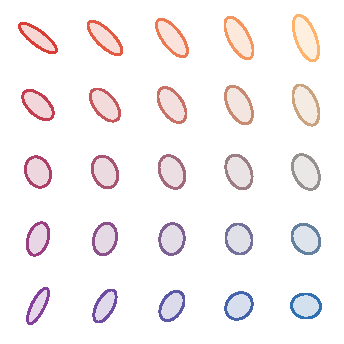
\includegraphics[width=.35\linewidth]{figures/barycenters-gaussian-covariances/moderate-grid.pdf} &
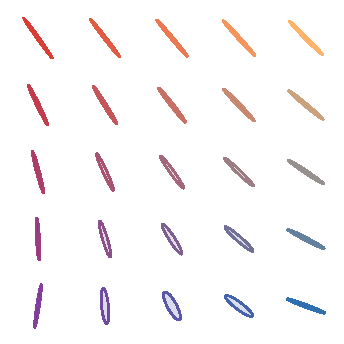
\includegraphics[width=.35\linewidth]{figures/barycenters-gaussian-covariances/anisotropic-grid.pdf}
\\[-.1em]
\small moderate anisotropy &
\small strong anisotropy
\end{tabular}
\caption{\emph{Bures--Wasserstein barycenters of centered Gaussian covariance matrices.} Each panel shows a $5\times5$ grid of barycenter ellipses for four corner covariances, without separate input panels: the corner ellipses are the four input covariances themselves. The right grid uses more anisotropic inputs, making the nonlinear rotation and scaling of covariance barycenters more visible.}
\index{Wasserstein!barycenter}% strictindex
\label{fig:barycenters-gaussian-covariances}
\end{figure}


%%%%%%%%%%%%%%%%%%%%%%%%%%%%%%%%%%%%%%%%%%%%%%%%%%%%%%%%%%%%%%%%%%%%%%%%%%%
\paragraph{Sinkhorn for barycenters.}
\index{Sinkhorn!barycenter}% strictindex

A key difference with the regularized two-marginal OT problem is that there is no canonical reference measure $\al\otimes\be$, because the barycenter $\al$ is unknown. To reduce complexity, one usually fixes a candidate support for the barycenter and solves the discrete problem~\eqref{eq-wass-discr}; this introduces a discretization error but keeps the number of unknowns manageable.
\index{discretization error}% strictindex
\index{reference!measure}% strictindex

One can then use the entropy-only convention of~\eqref{eq-regularized-discr} and approximate~\eqref{eq-wass-discr} by
\index{entropic!smoothing}% strictindex
\eql{\label{eq-entropic-bary}
	\umin{\a\in\simplex_n}
	\sum_{s=1}^S\la_s\MKD_{\C_s}^\epsilon(\a,\b_s)
}
for some $\epsilon>0$. This is a smooth convex minimization problem, which can be tackled using gradient descent~\cite{CuturiBarycenter}. An alternative is to use a descent method, typically quasi-Newton, on the semi-dual~\cite{2016-Cuturi-siims}; this is useful when adding extra regularization on the barycenter, for instance to impose smoothness.
\index{semi-dual}% strictindex

A simple but effective approach, developed in~\cite{2015-benamou-cisc}, observes that~\eqref{eq-entropic-bary} has the same minimizers as the weighted KL projection problem
\index{KL!projection}% strictindex
\eql{\label{eq-bary-entropy-couplings}
	\umin{(\P_s)_s}
	\enscond{
		\epsilon\sum_s\la_s\KLD(\P_s|\K_s)
	}{
		\foralls s,\ \transp{\P_s}\ones_n=\b_s,
		\quad
		\P_1\ones_{n_1}=\ldots=\P_S\ones_{n_S}
	},
}
where $\K_s\eqdef e^{-\C_s/\epsilon}$. The barycenter $\a$ is implicitly encoded in the common row marginal
\[
	\a=\P_1\ones_{n_1}=\ldots=\P_S\ones_{n_S}.
\]
The two objectives differ only by constants depending on $(\C_s,\epsilon)_s$, not on the couplings or on the barycenter. Assume below that every $\C_s$ is finite and every $\b_s$ is positive; zero-weight target atoms can be deleted before running the iteration. The optimal couplings solving~\eqref{eq-bary-entropy-couplings} then have scaling form
\index{optimal coupling}% strictindex
\index{scaling!form}% strictindex
\eql{\label{eq-bary-opt}
	\P_s=\diag(\uD_s)\K_s\diag(\vD_s),
}
and the generalized Sinkhorn iterations are
\index{Sinkhorn!iteration}% strictindex
\begin{align}
	\foralls s\in\range{1,S},\qquad
	\itt{\vD}_s
	&\eqdef
	\frac{\b_s}{\transp{\K_s}\it{\uD}_s},
	\label{eq-sinkhorn-bary}
	\\
	\foralls s\in\range{1,S},\qquad
	\itt{\uD}_s
	&\eqdef
	\frac{\itt{\a}}{\K_s\itt{\vD}_s},
	\label{eq-sinkhorn-bary-2}
	\\
	\qwhereq
	\itt{\a}
	&\eqdef
	\prod_s(\K_s\itt{\vD}_s)^{\la_s}.
	\label{eq-sinkhorn-bary-3}
\end{align}
The geometric mean in~\eqref{eq-sinkhorn-bary-3} enforces the fact that all couplings share the same barycenter marginal.

\begin{alg}[Entropic barycenter Sinkhorn]\label{alg:entropic-barycenter-sinkhorn}
\textbf{Input:} Finite costs $\C_s$, positive target histograms $\b_s$, barycenter weights $\lambda\in\operatorname{int}(\simplex_S)$, regularization $\epsilon>0$, tolerance $\mathrm{tol}$.

\textbf{Output:} Barycenter weights $\a$ and couplings $\P_s$.

\textbf{Initialize:} Set $\K_s=e^{-\C_s/\epsilon}$, $\uD_s^{(0)}=\ones_n$ for all $s$, \(r_0=+\infty\), and \(k=0\).

\textbf{While} \(r_k>\mathrm{tol}\) \textbf{do}:
\begin{algblock}

\textbf{Set} \(k\leftarrow k+1\).

\textbf{For} each marginal $s$ \textbf{do}
\begin{algblock}
\(\vD_s^{(k)} = \frac{\b_s}{\transp{\K_s}\uD_s^{(k-1)}}.\)
\end{algblock}
\textbf{Compute} barycenter marginal:
\(\a^{(k)} = \prod_s \bigl(\K_s\vD_s^{(k)}\bigr)^{\lambda_s}.\)

\textbf{For} each marginal $s$ \textbf{do}
\begin{algblock}
\(\uD_s^{(k)} = \frac{\a^{(k)}}{\K_s\vD_s^{(k)}}.\)
\end{algblock}

\textbf{Set} \(\P_s^{(k)}=\diag(\uD_s^{(k)})\K_s\diag(\vD_s^{(k)})\) for all \(s\).

\textbf{Set} \(r_k=\max_s \max\{\norm{\P_s^{(k)}\ones-\a^{(k)}}_1,\norm{(\P_s^{(k)})^\top\ones-\b_s}_1\}\).
\end{algblock}
\algreturnskip
\textbf{Return} \(\a^{(k)}\) and \(\P_s^{(k)}\).
\end{alg}

\begin{prop}[Dual of entropic barycenters]\label{prop-dual-entropic-barycenters}
\index{entropic!barycenter}% strictindex
	Under the preceding positivity assumptions, the optimal scalings in~\eqref{eq-bary-opt} can be written as $(\uD_s,\vD_s)=(e^{\fD_s/\epsilon},e^{\gD_s/\epsilon})$, where $(\fD_s,\gD_s)_s$ solve the dual problem
\index{dual!problem}% strictindex
	\eql{\label{eq-dual-bary-entropy}
		\umax{(\fD_s,\gD_s)_s}
		\enscond{
			\sum_s\la_s
				\left(
					\dotp{\gD_s}{\b_s}
					-\epsilon\dotp{\K_s e^{\gD_s/\epsilon}}{e^{\fD_s/\epsilon}}
					+\epsilon\sum_{i,j}(\K_s)_{i,j}
				\right)
		}{
			\sum_s\la_s\fD_s=0
		}.
	}
\end{prop}

\begin{proof}
	Introduce Lagrange multipliers in~\eqref{eq-bary-entropy-couplings}:
	\begin{align*}
		\umin{(\P_s)_s,\a}
		\umax{(\fD_s,\gD_s)_s}
		\sum_s\la_s\Big(
			\epsilon\KLD(\P_s|\K_s)
			+\dotp{\a-\P_s\ones_{n_s}}{\fD_s}
			+\dotp{\b_s-\transp{\P_s}\ones_n}{\gD_s}
		\Big).
	\end{align*}
	The explicit constraint $\a\in\simplex_n$ may be dropped here: nonnegativity of the couplings, together with $\P_s\ones_{n_s}=\a$ and $\transp{\P_s}\ones_n=\b_s$, already forces $\a\in\simplex_n$. We may therefore minimize the Lagrangian over $\a\in\RR^n$. Strong duality holds, so one can exchange the minimum and maximum. Finiteness of the minimum with respect to $\a$ gives the vector constraint $\sum_s\la_s\fD_s=0$, while minimization with respect to $\P_s$ gives the Legendre transform of $\KLD(\cdot|\K_s)$:
\index{duality!strong}% strictindex
\index{Legendre transform}% strictindex
	\[
		\umax{(\fD_s,\gD_s)_s}
		\sum_s\la_s
		\left[
			\dotp{\gD_s}{\b_s}
			-\epsilon
			\KLD^*\left(\frac{\fD_s\oplus\gD_s}{\epsilon}\middle|\K_s\right)
		\right],
		\qquad
		\sum_s\la_s\fD_s=0.
	\]
	The separable conjugate is
	\eql{\label{eq-legendre-kl-bary}
		\KLD^*(\VectMode{U}|\K)
		=
		\sum_{i,j}\K_{i,j}\big(e^{\VectMode{U}_{i,j}}-1\big),
	}
	because for $k>0$,
	\[
		\sup_{r\geq0}
		ur-\big(r\log(r/k)-r+k\big)
		=
		k(e^u-1),
	\]
		and the case $k=0$ follows by lower semicontinuity. Substituting this conjugate gives~\eqref{eq-dual-bary-entropy}, including its additive constant. The coordinate maximization in $\gD_s$ gives~\eqref{eq-sinkhorn-bary}; the block maximization in all $(\fD_s)_s$ under $\sum_s\lambda_s\fD_s=0$ gives the weighted geometric mean~\eqref{eq-sinkhorn-bary-3} and then~\eqref{eq-sinkhorn-bary-2}.
\index{lower semicontinuity}% strictindex
\end{proof}

Classical applications include two-dimensional image interpolation, three-dimensional shape interpolation, and barycenters on surfaces where the ground cost is the square of the geodesic distance; see~\cite{2015-solomon-siggraph} for applications to computer graphics and imaging.
\index{ground cost}% strictindex

\paragraph{Wasserstein-over-Wasserstein and barycenters.}
\index{law over measures}% strictindex
\index{random probability measure}% strictindex
\index{nonlinear flattening}% strictindex
The barycenter formula does not require a finite list of inputs. The Wasserstein-over-Wasserstein viewpoint of Section~\ref{sec-wasserstein-over-wasserstein} makes it possible to replace the discrete family $(\be_s,\la_s)_s$ by a law $\mathfrak A\in\Pp(\Pp(\Omega))$ over probability measures. Assume, for instance, that $c$ is lower semicontinuous and that there exists at least one $\beta_0\in\Pp(\Omega)$ with
\[
\int_{\Pp(\Omega)}\MK_c(\beta_0,\alpha)\d\mathfrak A(\alpha)<+\infty,
\]
together with the usual compactness or coercivity hypotheses ensuring existence of minimizers. For instance, these assumptions are automatic when $\Omega$ is compact and $c$ is continuous. The barycenter correspondence is then
\index{Wasserstein!over Wasserstein}% strictindex
\index{Wasserstein!barycenter}% strictindex
\index{flattening map}% strictindex
\[
\mathcal B_c(\mathfrak A)
\eqdef
\operatorname*{Argmin}_{\beta\in\Pp(\Omega)}
\int_{\Pp(\Omega)}\MK_c(\beta,\alpha)\d\mathfrak A(\alpha).
\]
When this set is a singleton, we denote its element by
\[
\widetilde\alpha_{\mathfrak A}
\eqdef
\uargmin{\beta\in\Pp(\Omega)}
\int_{\Pp(\Omega)}\MK_c(\beta,\alpha)\d\mathfrak A(\alpha),
\]
which defines a nonlinear flattening map $\mathfrak A\mapsto\widetilde\alpha_{\mathfrak A}$ from laws over measures back to measures on $\Omega$.
When $\mathfrak A=\sum_s\la_s\delta_{\be_s}$, this is exactly the finite barycenter problem above. This map should be contrasted with the linear collapsed, or barycentric, mixture $\bar\alpha_{\mathfrak A}$ of Definition~\ref{def-collapsed-barycentric-mixture}, which simply averages the input measures themselves. The two operations agree in degenerate linear situations, but in general $\widetilde\alpha_{\mathfrak A}$ is a geometric average in transport space, whereas $\bar\alpha_{\mathfrak A}$ is an ordinary mixture in the ambient linear space of measures.
\index{collapsed mixture}% strictindex
\index{barycentric!mixture}% strictindex

\index{barycenter!law of large numbers}% strictindex
\index{random measure}% strictindex
The next result records the corresponding law of large numbers. It is useful when a dataset is itself made of probability measures, for instance populations of histograms, posterior distributions or shapes. We state it in the compact setting, where no moment or tightness side conditions are needed; non-compact extensions require the usual integrability assumptions. Consistency of Wasserstein barycenters and related statistical constructions is developed in~\cite{boissard2015distribution,leGouic2016existence,zemel2017fr}; streaming and large-scale uses of many input measures appear for instance in~\cite{staib2017parallel,srivastava2015wasp,srivastava2018scalable}.
\index{law of large numbers}% strictindex
\index{Wasserstein!barycenter!consistency}% strictindex
\index{empirical!measure over measures}% strictindex

\begin{prop}[Law of large numbers for barycenters over measures]\label{prop-wow-barycenter-lln}
	Let $\Omega$ be a compact metric space, let $c:\Omega\times\Omega\to\RR$ be continuous, and let $\mathfrak A\in\Pp(\Pp(\Omega))$. Let $\alpha_1,\alpha_2,\ldots$ be independent random probability measures with common law $\mathfrak A$, and set
	\[
		\widehat{\mathfrak A}_p
		\eqdef
		\frac1p\sum_{i=1}^p\delta_{\alpha_i}
		\in\Pp(\Pp(\Omega)).
	\]
	Then, almost surely,
	\[
		\widehat{\mathfrak A}_p \rightharpoonup \mathfrak A
		\quad\text{in }\Pp(\Pp(\Omega)),
		\qquad
		\bar\alpha_{\widehat{\mathfrak A}_p}
		\rightharpoonup
		\bar\alpha_{\mathfrak A}
		\quad\text{in }\Pp(\Omega).
	\]
	Moreover, if $\mathcal B_c(\mathfrak A)=\{\widetilde\alpha_{\mathfrak A}\}$ is a singleton and if $\widetilde\alpha_{\widehat{\mathfrak A}_p}\in\mathcal B_c(\widehat{\mathfrak A}_p)$ is any empirical barycenter, then, almost surely,
	\[
		\widetilde\alpha_{\widehat{\mathfrak A}_p}
		\rightharpoonup
		\widetilde\alpha_{\mathfrak A}
		\quad\text{in }\Pp(\Omega).
	\]
\end{prop}

\begin{proof}
	Set $K=\Pp(\Omega)$. Since $\Omega$ is compact metric, $K$ is compact metric for weak convergence, and so is $\Pp(K)$. The space $\Cc(K)$ is separable for the uniform norm. Applying the scalar strong law to a countable dense family of test functions and then using uniform approximation gives, almost surely, for every $\Phi\in\Cc(K)$,
	\[
		\int \Phi(\alpha)\d\widehat{\mathfrak A}_p(\alpha)
		=
		\frac1p\sum_{i=1}^p\Phi(\alpha_i)
		\longrightarrow
		\int \Phi(\alpha)\d\mathfrak A(\alpha)
	\]
	This is exactly $\widehat{\mathfrak A}_p\rightharpoonup\mathfrak A$ in $\Pp(K)$.

	For the collapsed mixtures, take $f\in\Cc(\Omega)$ and define $\Phi_f(\alpha)=\int_\Omega f\d\alpha$. This function is continuous on $\Pp(\Omega)$. Hence
	\[
		\int_\Omega f\d\bar\alpha_{\widehat{\mathfrak A}_p}
		=
		\int_{\Pp(\Omega)}\Phi_f(\alpha)\d\widehat{\mathfrak A}_p(\alpha)
		\longrightarrow
		\int_{\Pp(\Omega)}\Phi_f(\alpha)\d\mathfrak A(\alpha)
		=
		\int_\Omega f\d\bar\alpha_{\mathfrak A},
	\]
	which proves $\bar\alpha_{\widehat{\mathfrak A}_p}\rightharpoonup\bar\alpha_{\mathfrak A}$.

	It remains to prove the nonlinear barycenter consistency. Since $c$ is continuous on the compact product $\Omega\times\Omega$, the value $(\beta,\alpha)\mapsto\MK_c(\beta,\alpha)$ is continuous on $K^2$. Therefore the map $\beta\mapsto h_\beta$, where $h_\beta(\alpha)=\MK_c(\beta,\alpha)$, is continuous from the compact space $K$ to $\Cc(K)$. Its image
	\[
		\mathcal H
		\eqdef
		\{h_\beta:\beta\in K\}
	\]
	is compact in $\Cc(K)$. The convergence of $\widehat{\mathfrak A}_p$ to $\mathfrak A$ is uniform over $\mathcal H$: given $\eta>0$, cover $\mathcal H$ by finitely many $\eta$-balls in $\norm{\cdot}_\infty$, use weak convergence for the centers, and bound the error on the balls by the total variation of $\widehat{\mathfrak A}_p-\mathfrak A$. Hence the empirical objectives
	\[
		F_p(\beta)\eqdef\int\MK_c(\beta,\alpha)\d\widehat{\mathfrak A}_p(\alpha)
	\]
	converge uniformly on $K$ to
	\[
		F(\beta)\eqdef\int\MK_c(\beta,\alpha)\d\mathfrak A(\alpha).
	\]
	Let $\beta_p\in\mathcal B_c(\widehat{\mathfrak A}_p)$. Compactness gives a subsequence $\beta_{p_k}\rightharpoonup\beta$. Uniform convergence, continuity of $F$, and optimality of $\beta_{p_k}$ give, for any $\gamma\in K$,
	\[
		F(\beta)
		=
		\lim_k F_{p_k}(\beta_{p_k})
		\leq
		\lim_k F_{p_k}(\gamma)
		=
		F(\gamma),
	\]
	so $\beta\in\mathcal B_c(\mathfrak A)$. If this set is the singleton $\{\widetilde\alpha_{\mathfrak A}\}$, every converging subsequence has the same limit, and therefore the whole sequence $\widetilde\alpha_{\widehat{\mathfrak A}_p}$ converges to $\widetilde\alpha_{\mathfrak A}$.
\end{proof}

The first convergence above is a classical law of large numbers applied to random elements of the Wasserstein space. The second, for $\bar\alpha_{\widehat{\mathfrak A}_p}$, is still linear after testing against $f\in\Cc(\Omega)$. The third convergence is its nonlinear counterpart: one first forms an empirical law over measures and then solves a Wasserstein barycenter problem. The number $p$ of input measures should not be confused with the number $n$ of samples used to approximate each input measure, studied in Section~\ref{sec-sample-complexity}. In applications one often observes $p$ empirical measures, each made of roughly $n$ atoms, hence about $np$ points in total. Balancing the error due to finitely many input laws against the error due to finitely sampled input laws is a separate statistical and computational tradeoff.
\index{sample complexity}% strictindex
\index{statistical optimal transport}% strictindex

\paragraph{Toward central limit theorems on Wasserstein space.}
\index{Wasserstein!space CLT}% strictindex
\index{tangent coordinate}% strictindex
\index{cylindrical Gaussian}% strictindex

The same hierarchy suggests a central-limit refinement of the preceding law of large numbers, but the nonlinear geometry makes this substantially more delicate. For the linear collapse $\bar\alpha_{\widehat{\mathfrak A}_p}$, testing against a fixed $f\in\Cc(\Omega)$ reduces the question to the classical scalar central limit theorem for the random variable $\alpha\mapsto\int f\d\alpha$. For the nonlinear barycenter $\widetilde\alpha_{\widehat{\mathfrak A}_p}$, however, there is no canonical vector difference $\widetilde\alpha_{\widehat{\mathfrak A}_p}-\widetilde\alpha_{\mathfrak A}$ inside $\Pp(\Omega)$. One has to choose a local linearization. When the population barycenter is sufficiently regular so that the optimal map $T_p$ from $\widetilde\alpha_{\mathfrak A}$ to $\widetilde\alpha_{\widehat{\mathfrak A}_p}$ exists, this amounts to asking whether $\sqrt p\,(T_p-\Id)$ converges in a Hilbert space such as $L^2(\widetilde\alpha_{\mathfrak A})$. In nonsmooth settings one must instead work with optimal-plan or logarithmic-map coordinates. Even after such a linearization, an infinite-dimensional CLT requires tightness of the rescaled tangent variables and a genuine Radon Gaussian random element; in a Hilbert space, the associated covariance must be trace class. A cylindrical Gaussian limit alone is therefore not a probability law on the tangent space. This obstruction explains why Wasserstein-space CLTs are more rigid than the weak laws above.
\index{central limit theorem}% strictindex
\index{Wasserstein!barycenter}% strictindex

There are nevertheless important settings where such results can be proved. In one dimension, the quantile representation linearizes $\Wass_2$, so barycenter fluctuations can be studied through empirical averages of quantile functions. Another finite-dimensional case is the family of non-degenerate Gaussian measures in fixed dimension, where $\Wass_2$ reduces to the Bures geometry of means and covariance matrices. Agueh and Carlier~\cite{agueh2017vers} formulate this Wasserstein-barycenter CLT precisely in tangent coordinates and prove it in a few special cases, including the one-dimensional non-atomic setting and finite laws supported on non-degenerate Gaussian measures. Entropic barycenters give a smoother variant for which central-limit theorems for empirical barycenters are also available~\cite{CarlierEichingerKroshnin2020EntropicBarycenterCLT}. These results should be read as nonlinear analogues of the statistical limits discussed in Chapter~\ref{sec-statistical-ot}, not as a generic Hilbert-space CLT valid on all of $\Pp(\Omega)$.
\index{quantile!function}% strictindex
\index{Bures!metric}% strictindex

\section{Multimarginal OT}
\index{multi-marginal!OT}% strictindex
\label{sec-multimarginal-ot}
\label{subsec:multi-marginal}

Multi-marginal OT couples more than two measures at once. It is the natural language for barycenters, matching with teams and several-body costs, but its tensor dimension is the main computational obstacle.

\paragraph{Definition and basic structure.}

The multi-marginal formulation replaces a coupling between two measures by a joint distribution with several prescribed marginals. Given measures $(\al_s)_{s=1}^S$ on spaces $(\Xx_s)_{s=1}^S$ and a lower-semicontinuous cost $c:\Xx_1\times\cdots\times\Xx_S\to\RR\cup\{+\infty\}$ bounded from below, the problem reads
\index{multi-marginal!OT}% strictindex
\[
	\inf_{\pi\in\Couplings(\al_1,\ldots,\al_S)}
	\int_{\Xx_1\times\cdots\times\Xx_S}
	c(x_1,\ldots,x_S)\d\pi(x_1,\ldots,x_S),
\]
where $\Couplings(\al_1,\ldots,\al_S)$ is the set of probability measures whose $s$-th marginal is $\al_s$. This is still a linear program in the discrete setting, but its ambient tensor has size $\prod_s n_s$.
\index{probability measure}% strictindex

\paragraph{Monge structure and splitting-set twist.}
\index{twist on splitting sets}% strictindex
\index{multi-marginal!Monge map}% strictindex
\index{splitting set}% strictindex

As in the two-marginal case, one would like to know when the optimal joint law is induced by deterministic maps from one marginal. The relevant non-degeneracy assumption is stronger than pairwise twist, because the other $S-1$ variables have to be recovered simultaneously. The condition below is the standard multi-marginal analogue used in the Monge-structure theory of Gangbo--Swiech and Pass~\cite{GangboSciech,Pass2,PassMultiMarginalStructure,PassMultiReview}.
\index{twist condition}% strictindex

\begin{defn}[Twist on splitting sets]\label{def-twist-splitting-sets}
	Fix $x_1\in\Xx_1$. A set $M\subset\Xx_2\times\cdots\times\Xx_S$ is a $c$-splitting set at $x_1$ if there exist functions $u_s:\Xx_s\to\RR\cup\{-\infty\}$, for $s=2,\ldots,S$, such that
	\[
		\sum_{s=2}^S u_s(x_s)\leq c(x_1,x_2,\ldots,x_S)
	\]
	for all $(x_2,\ldots,x_S)$, with equality on $M$. Assume $c$ is differentiable in $x_1$. The cost is twisted on splitting sets if, for every $x_1$ and every $c$-splitting set $M$ at $x_1$, the map
	\[
		(x_2,\ldots,x_S)
		\longmapsto
		\nabla_{x_1}c(x_1,x_2,\ldots,x_S)
	\]
	is injective on $M$.
\index{c-splitting set}% strictindex
\end{defn}

\begin{prop}[Multi-marginal Monge structure]\label{prop-multimarginal-monge-structure}
\index{multi-marginal!Monge map}% strictindex
\index{twist on splitting sets}% strictindex
	Assume that $\Xx_s\subset\RR^d$, that $c$ is continuous and differentiable with respect to $x_1$, and that $c$ is twisted on splitting sets. Suppose that Kantorovich dual maximizers $(\varphi_s)_{s=1}^S$ exist, that $\al_1$ is absolutely continuous, and that $\varphi_1$ is differentiable $\al_1$-a.e. Then every optimal plan $\pi^\star\in\Couplings(\al_1,\ldots,\al_S)$ is concentrated on the graph of maps
\index{splitting set}% strictindex
	\[
		\pi^\star=(\Id,\T_2,\ldots,\T_S)_\sharp\al_1,
		\qquad
		(\T_s)_\sharp\al_1=\al_s.
	\]
	In particular, under these hypotheses the optimizer is unique.
\index{Kantorovich!potential}% strictindex
\index{absolute continuity}% strictindex
\end{prop}
\begin{proof}
	Let $(\varphi_s)_{s=1}^S$ be optimal dual potentials. Complementary slackness gives a Borel contact set $\Gamma$ of full $\pi^\star$-measure on which $\sum_s\varphi_s(x_s)=c(x_1,\ldots,x_S)$. After disintegrating with respect to the first marginal, fix a point $x_1$ where $\varphi_1$ is differentiable and where the conditional plan is concentrated on the fiber
	\[
		M(x_1)=\{(x_2,\ldots,x_S):(x_1,x_2,\ldots,x_S)\in\Gamma\}.
	\]
	For this fixed $x_1$, the fiber is a splitting set. Indeed, set $u_2=\varphi_2+\varphi_1(x_1)$ and $u_s=\varphi_s$ for $s\geq3$. Dual feasibility gives $\sum_{s=2}^S u_s(x_s)\leq c(x_1,x_2,\ldots,x_S)$, and equality holds on $M(x_1)$. If $(x_2,\ldots,x_S)\in M(x_1)$, the function
	\[
		z\longmapsto c(z,x_2,\ldots,x_S)-\sum_{s=2}^S\varphi_s(x_s)
	\]
	touches $\varphi_1$ from above at $z=x_1$. Differentiating at this contact point gives
	\[
		\nabla\varphi_1(x_1)=\nabla_{x_1}c(x_1,x_2,\ldots,x_S).
	\]
	All points in the fiber therefore have the same value of $\nabla_{x_1}c$. Twist on splitting sets makes the fiber a singleton for $\al_1$-a.e. $x_1$. Disintegrating $\pi^\star$ with respect to its first marginal gives Dirac conditional measures, hence measurable maps $(\T_2,\ldots,\T_S)$. If $\pi^1$ and $\pi^2$ are two optimal plans, their average is also optimal. The conditional measure of this average over $x_1$ is the average of the two Dirac conditionals, and it must again be a Dirac mass by the preceding argument. Hence the two Dirac masses coincide for $\al_1$-a.e. $x_1$, proving uniqueness.
\index{disintegration}% strictindex
\index{Dirac measure}% strictindex
\end{proof}

\paragraph{Coulomb cost and density-functional theory.}
\index{Coulomb cost}% strictindex
\index{density-functional theory}% strictindex

A second canonical example, besides barycenters, comes from electronic structure. For $N$ electrons in $\RR^3$, the repulsive Coulomb interaction is the multi-body cost
\[
	c_{\mathrm{Coul}}(x_1,\ldots,x_N)
	\eqdef
	\sum_{1\leq i<j\leq N}\frac{1}{\norm{x_i-x_j}},
\]
with the value $+\infty$ on the collision set. This lower-semicontinuous singularity is not a harmless detail: finite-energy plans avoid electron collisions, and the smooth structure theorem above should be read as a guide rather than as a global theorem for the Coulomb cost. If $\rho$ is an electron density with $\int_{\RR^3}\rho(x)\d x=N$ and $\al=\rho/N$ is the associated probability density, the strictly-correlated-electrons relaxation of density-functional theory is the equal-marginal problem
\index{Coulomb cost}% strictindex
\[
	V_{\mathrm{ee}}^{\mathrm{SCE}}[\rho]
	\eqdef
	\inf_{\pi\in\Couplings(\al,\ldots,\al)}
	\int_{(\RR^3)^N}
	c_{\mathrm{Coul}}(x_1,\ldots,x_N)
	\d\pi(x_1,\ldots,x_N).
\]
Since the cost and constraints are permutation invariant, symmetrizing any admissible plan does not change its value, so one may equivalently minimize over symmetric plans. This functional gives the smallest possible electron--electron repulsion compatible with the prescribed one-particle density; it appears as the strong-interaction limit in density-functional theory and was connected to optimal transport in~\cite{GorSeiVig,BuDePGor,CotarDFT,DiMarinoGerolinNennaRepulsiveCosts}. The deterministic ansatz writes a plan through co-motion maps
\index{density-functional theory}% strictindex
\index{co-motion function}% strictindex
\[
	\pi=(\Id,\T_2,\ldots,\T_N)_\sharp\al,
	\qquad
	(\T_i)_\sharp\al=\al,
\]
so that the position of one electron determines the positions of the others. The following cyclic version is the most common structural form of this ansatz in the strictly-correlated-electrons literature.
\index{strictly correlated electrons}% strictindex
\index{co-motion map}% strictindex
\index{equal marginal}% strictindex
\index{symmetric plan}% strictindex
\index{electron density}% strictindex

\begin{prop}[Cyclic co-motion plans]\label{prop-cyclic-comotion-plans}
\index{cyclic!co-motion plan}% strictindex
	Let $\al\in\Pp(\RR^3)$ and let $\T:\RR^3\to\RR^3$ be measurable with $\T_\sharp\al=\al$ and $\T^N=\Id$ $\al$-a.e. Set $\T^0=\Id$ and
	\[
		\pi_\T=(\T^0,\T^1,\ldots,\T^{N-1})_\sharp\al .
	\]
	Then $\pi_\T\in\Couplings(\al,\ldots,\al)$. If $R_\sigma(x_1,\ldots,x_N)=(x_{\sigma(1)},\ldots,x_{\sigma(N)})$ for $\sigma\in\Perm(N)$, then
	\[
		\bar\pi_\T\eqdef\frac1{N!}\sum_{\sigma\in\Perm(N)}(R_\sigma)_\sharp\pi_\T
	\]
	is a symmetric admissible plan and
	\[
		\int c_{\mathrm{Coul}}\d\bar\pi_\T
		=
		\int c_{\mathrm{Coul}}\d\pi_\T
		=
		\int_{\RR^3}
		\sum_{0\leq i<j\leq N-1}
		\frac{1}{\norm{\T^i(x)-\T^j(x)}}\d\al(x).
	\]
\end{prop}
\begin{proof}
	Since $\T_\sharp\al=\al$, all iterates $\T^i$ preserve $\al$, so every marginal of $\pi_\T$ is $\al$. The plan $\bar\pi_\T$ is an average of coordinate permutations of $\pi_\T$, hence has the same marginals and is invariant under coordinate permutations. The Coulomb cost is symmetric in its arguments, so its integral is unchanged by each $R_\sigma$. The last identity follows by evaluating $c_{\mathrm{Coul}}$ on the graph $(x,\T(x),\ldots,\T^{N-1}(x))$.
\index{Coulomb cost}% strictindex
\index{symmetric plan}% strictindex
\end{proof}

Proposition~\ref{prop-multimarginal-monge-structure} explains the general mechanism that can force graph solutions, while Proposition~\ref{prop-cyclic-comotion-plans} records the additional equal-marginal symmetry used by co-motion maps. For the Coulomb cost, however, the singular repulsion and permutation symmetry make the structure delicate: co-motion maps are optimal in special geometries, but they are not universally optimal, and counterexamples are known~\cite{ColomboStraCoulombCounterexamples,BindiniDePascaleKausamoDeterministicCoulomb}. Thus the DFT problem is both a central application and a warning that multi-marginal OT is richer than a naive deterministic matching problem.
\index{co-motion map}% strictindex
\index{counterexample}% strictindex

Figure~\ref{fig:multimarginal-coulomb-sinkhorn} shows the same phenomenon in a deliberately small one-dimensional model. Three identical two-bump marginals, with unequal component masses and widths, interact through a softened pairwise Coulomb cost. The displayed object is the two-particle marginal of the entropic three-marginal optimizer, with its one-dimensional marginals glued to the top and right sides of the plan. As $\epsilon$ decreases, mass is pushed away from the collision diagonal $x_1=x_2$, revealing the repulsive geometry that underlies the strictly-correlated-electrons model.
\index{Coulomb cost}% strictindex

\begin{figure}[H]
\centering
\begin{tabular}{@{}ccc@{}}
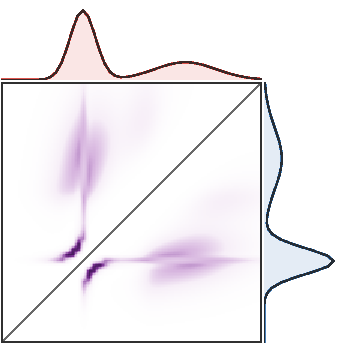
\includegraphics[width=.30\linewidth]{figures/multimarginal-coulomb-sinkhorn/epsilon-small.pdf} &
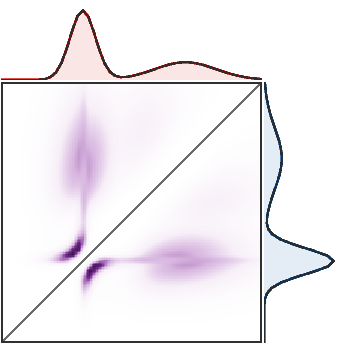
\includegraphics[width=.30\linewidth]{figures/multimarginal-coulomb-sinkhorn/epsilon-medium.pdf} &
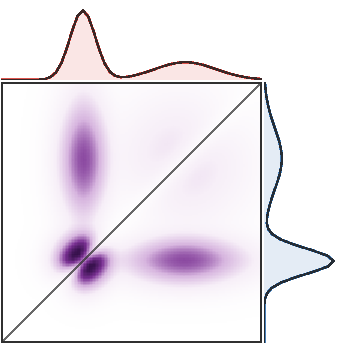
\includegraphics[width=.30\linewidth]{figures/multimarginal-coulomb-sinkhorn/epsilon-large.pdf}
\\[-.1em]
\small $\epsilon=0.06$ & \small $\epsilon=0.16$ & \small $\epsilon=0.50$
\end{tabular}
\caption{\emph{Entropic three-marginal Coulomb transport in one dimension.} The three marginals are the same asymmetric two-Gaussian mixture, and the pairwise cost is $((x_r-x_s)^2+\delta^2)^{-1/2}$. Each panel shows the $(X_1,X_2)$ marginal of the tensor Sinkhorn solution; the red top strip and blue right strip are the prescribed marginals, while the thin dark curves are the marginals obtained by summing the displayed pairwise plan. Small regularization concentrates the plan away from the collision diagonal, while larger regularization blurs the repulsive arrangement toward the independent reference.}
\index{Coulomb cost}% strictindex
\index{multi-marginal!Sinkhorn}% strictindex
\index{density-functional theory}% strictindex
\label{fig:multimarginal-coulomb-sinkhorn}
\end{figure}

\paragraph{Multi-marginal formulation of barycenters.}
\index{multi-marginal!OT}% strictindex
\index{multi-marginal!formulation}% strictindex

Wasserstein barycenters are the central example. For the squared Euclidean cost, one can introduce a latent barycenter point and eliminate it explicitly, leading to the multi-marginal cost
\index{multi-marginal!cost}% strictindex
\index{Wasserstein!barycenter}% strictindex
\[
	c_{\mathrm{bar}}(x_1,\ldots,x_S)
	=
	\min_{x\in\RR^d}
	\sum_{s=1}^S\la_s\norm{x-x_s}^2.
\]

\begin{prop}[Multi-marginal formula for quadratic barycenters]\label{prop-multimarginal-barycenter}
\index{multi-marginal!OT}% strictindex
\index{quadratic!barycenter}% strictindex
	Let $\be_1,\ldots,\be_S\in\Pp_2(\RR^d)$ and $\la\in\simplex_S$. Define
	\[
		B(x_1,\ldots,x_S)=\sum_{s=1}^S\la_s x_s,
		\qquad
		c_{\mathrm{bar}}(x_1,\ldots,x_S)=\min_x\sum_s\la_s\norm{x-x_s}^2.
	\]
	If $\pi^\star$ solves the multi-marginal OT problem with marginals $(\be_s)_s$ and cost $c_{\mathrm{bar}}$, then $\al^\star=B_\sharp\pi^\star$ is a Wasserstein barycenter. Conversely, every barycenter is obtained this way from an optimal multi-marginal plan.
\index{Wasserstein!barycenter}% strictindex
\index{multi-marginal!OT}% strictindex
\end{prop}

\begin{proof}
	For any candidate barycenter $\al$ and couplings $\pi_s\in\Couplings(\al,\be_s)$, glue the couplings along their common $\al$ marginal to obtain a joint law of $(X,Y_1,\ldots,Y_S)$. Conditioning on $(Y_s)_s$ and minimizing over $X$ gives
\index{joint!law}% strictindex
	\[
		\sum_s\la_s\EE\norm{X-Y_s}^2
		\geq
		\EE\min_x\sum_s\la_s\norm{x-Y_s}^2
		=
		\EE c_{\mathrm{bar}}(Y_1,\ldots,Y_S).
	\]
	Taking the infimum over the couplings gives that the barycenter value is at least the multi-marginal value. Conversely, from an optimal multi-marginal plan $\pi^\star$, set $X=B(Y_1,\ldots,Y_S)$. The couplings between $X$ and each $Y_s$ are feasible for the barycenter problem and attain exactly the multi-marginal cost, proving equality and the formula.
\index{multi-marginal!cost}% strictindex
	If $\al^\star$ is any barycenter, choose optimal couplings between $\al^\star$ and each $\be_s$ and glue them along the common $\al^\star$ marginal. Since the barycenter and multi-marginal values are equal, the conditional minimization inequality above must be an equality. Thus $X=B(Y_1,\ldots,Y_S)$ almost surely for the induced optimal multi-marginal plan, and $\al^\star=B_\sharp\pi^\star$.
\index{optimal coupling}% strictindex
\index{multi-marginal!OT}% strictindex
\end{proof}

\begin{cor}[Gaussian and discrete barycenters]\label{cor-gaussian-discrete-barycenters}
\index{Gaussian!barycenter}% strictindex
\index{discrete!barycenter}% strictindex
	For Gaussian input measures, there exists a Gaussian quadratic Wasserstein barycenter. If at least one positive-weight input has positive-definite covariance, the barycenter is unique and is therefore Gaussian. If the input measures are discrete, then there exists a barycenter supported on the set of weighted averages $\sum_s\la_s x_{s,i_s}$ of one support point from each input; in particular, if the $s$-th input has $n_s$ atoms, a barycenter exists with at most $\prod_s n_s$ atoms.
\index{Wasserstein!barycenter}% strictindex
\index{Gaussian!measure}% strictindex
\end{cor}

\begin{proof}
	Let the input Gaussians have means $\mean_s$ and covariances $\cov_s$. For any candidate barycenter $\al$ with mean $\mean$ and covariance $\cov$, Gelbrich's inequality~\cite{gelbrich1990formula}, proved later in Theorem~\ref{thm-gelbrich-projection}, gives
	\[
		\Wass_2^2(\al,\be_s)
		\geq
		\norm{\mean-\mean_s}^2+\Bb(\cov,\cov_s)^2,
	\]
		with equality for a Gaussian law with mean $\mean$ and covariance $\cov$. Therefore the barycenter objective is bounded below by a function depending only on $(\mean,\cov)$, and this lower bound is attained by a Gaussian measure with minimizing mean and covariance. This proves existence of a Gaussian barycenter. If one active input covariance is positive definite, that input is absolutely continuous, so the uniqueness criterion stated after~\eqref{eq-barycenter-generic} shows that every barycenter coincides with this Gaussian one. For discrete inputs, any multi-marginal optimizer is supported on the finite product of the input supports, and $B$ maps this product to at most $\prod_s n_s$ points.
\index{Gaussian!barycenter}% strictindex
\index{Gaussian!measure}% strictindex
\index{multi-marginal!OT}% strictindex
\end{proof}

\paragraph{Entropic regularization of multi-marginal OT.}
\index{entropic!regularization}% strictindex

As in the two-marginal case, adding an entropic penalty with respect to the product measure $\al_1\otimes\cdots\otimes\al_S$ leads to scaling algorithms:
\index{scaling!algorithm}% strictindex
\index{product!measure}% strictindex
\[
	\inf_{\pi\in\Couplings(\al_1,\ldots,\al_S)}
	\int c\d\pi+\epsilon\KL(\pi|\al_1\otimes\cdots\otimes\al_S).
\]
The optimizer has the generalized Gibbs form
\[
	\d\pi^\star(x_1,\ldots,x_S)
	=
	\exp\!\left(\frac{\sum_s f_s(x_s)-c(x_1,\ldots,x_S)}{\epsilon}\right)
	\prod_s\d\al_s(x_s),
\]
and generalized Sinkhorn iterations alternately update one potential $f_s$ so that the $s$-th marginal is correct. This formula is direct but, without additional structure, it is mostly a conceptual baseline. In the discrete case, even storing the Gibbs tensor or the coupling requires $\prod_s n_s$ entries, and the unstructured multi-marginal Sinkhorn complexity inherits this exponential dependence on the number of marginals~\cite{LinHoCuturiJordan2022MOTComplexity}.

The important exception is when the cost has a sparse graphical structure. If, for instance,
\[
	c(x_1,\ldots,x_S)=\sum_{(r,s)\in E} c_{r,s}(x_r,x_s),
\]
then the tensor contractions needed by Sinkhorn can be organized by message passing on the graph $G=(\{1,\ldots,S\},E)$. The complexity is then controlled by the treewidth of $G$ rather than by the full tensor dimension: trees and, more generally, small-treewidth graphs require only clique tensors of bounded order. This viewpoint connects entropic multi-marginal OT with probabilistic graphical models and Schr\"odinger bridge computations~\cite{HaaslerRinghChenKarlsson2021TreeMOT,HaaslerSinghZhangKarlssonChen2020PGMMOT,FanHaaslerKarlssonChen2021GraphCostMOT,AltschulerBoixAdsera2022StructuredMOT}. A representative fluid-mechanics example is the time discretization of Brenier's generalized incompressible Euler problem: the kinetic action couples neighboring time slices and the periodic incompressibility constraint closes the chain into a cycle, a graph of treewidth two. Entropic Bregman/Sinkhorn schemes exploit exactly this circular structure~\cite{2015-benamou-cisc,BenamouCarlierNenna2018GeneralizedIncompressible}.
\index{Sinkhorn!iteration}% strictindex
\index{treewidth}% strictindex
\index{graphical model}% strictindex
\index{message passing}% strictindex
\index{incompressible Euler}% strictindex

Practical barycenter solvers therefore exploit separability of the cost, low-rank structure, convolutional kernels, or a fixed barycenter support.
\index{low-rank!optimal transport}% strictindex

In finite dimension, the direct generalized scaling scheme is the tensor version of Sinkhorn. The explicit algorithm below assumes positive marginals and a finite cost tensor; forbidden configurations with infinite cost can instead be removed from the tensor support, provided the remaining marginal constraints are feasible.

\begin{alg}[Multi-marginal Sinkhorn]\label{alg:multimarginal-sinkhorn}
\textbf{Input:} Positive marginals $\a_s\in\simplex_{n_s}$, finite tensor cost $C$, regularization $\epsilon>0$, tolerance $\mathrm{tol}$.

\textbf{Output:} Multi-marginal entropic coupling tensor $P$.

\textbf{Build}
\(K_{i_1,\ldots,i_S} = \exp\!\left(-\frac{C_{i_1,\ldots,i_S}}{\epsilon}\right) \prod_{s=1}^S(\a_s)_{i_s}.\)

\textbf{Initialize:} Set \(u_s=\ones_{n_s}\) for all $s$ and residual \(r=+\infty\).

\textbf{While} \(r>\mathrm{tol}\) \textbf{do}:
\begin{algblock}

\textbf{For} $s=1,\ldots,S$ \textbf{do}:
\begin{algblock}
\((u_s)_i \leftarrow \frac{(\a_s)_i} { \sum_{i_1,\ldots,i_{s-1},i_{s+1},\ldots,i_S} K_{i_1,\ldots,i_{s-1},i,i_{s+1},\ldots,i_S} \prod_{r\neq s}(u_r)_{i_r}}.\)
\end{algblock}

\textbf{Set} \(P_{i_1,\ldots,i_S}=K_{i_1,\ldots,i_S}\prod_s (u_s)_{i_s}\).

\textbf{Set} \(r=\max_s\norm{(\mathrm{proj}_s)_\sharp P-\a_s}_1\).
\end{algblock}
\algreturnskip
\textbf{Return} \(P\).
\end{alg}


%%%%%%%%%%%%%%%%%%%%%%%%%%%%%%%%%%%%%%%%%%%%%%%%%%%%%%%%%%%%%%%%%%%%%%%%%%%
%%%%%%%%%%%%%%%%%%%%%%%%%%%%%%%%%%%%%%%%%%%%%%%%%%%%%%%%%%%%%%%%%%%%%%%%%%%
%%%%%%%%%%%%%%%%%%%%%%%%%%%%%%%%%%%%%%%%%%%%%%%%%%%%%%%%%%%%%%%%%%%%%%%%%%%
\section{Low-Rank Optimal Transport}
\index{low-rank!optimal transport}% strictindex
\label{sec-low-rank-ot}
\index{factored coupling}% strictindex

Low-rank OT reduces the size of a transport plan by forcing the coupling itself to pass through a small latent measure. This is useful when the mass exchange is expected to be organized by a few hidden clusters or prototypes, and it is distinct from approximating the Sinkhorn kernel by a low-rank matrix. The idea was introduced statistically through factored couplings by Forrow, H\"utter, Nitzan, Rigollet, Schiebinger and Weed~\cite{forrow2019factored}, and developed algorithmically for arbitrary costs by Scetbon, Cuturi and Peyr\'e~\cite{scetbon2021lowrank}.
\index{latent measure}% strictindex
\index{Sinkhorn!low-rank}% strictindex

\Needspace{18\baselineskip}
\begin{defn}[Low-rank factored couplings]\label{def-low-rank-couplings}
\index{low-rank!coupling}% strictindex
\index{nonnegative rank}% strictindex
	Let $\a\in\simplex_n$, $\b\in\simplex_m$ and let $r\geq1$. A rank-$r$ factored coupling is a triple $(Q,R,g)$ such that
	\[
		Q\in\RR_+^{n\times r},\qquad
		R\in\RR_+^{m\times r},
		\qquad g\in\simplex_r,
	\]
	with
	\[
		Q\ones_r=\a,
		\qquad
		R\ones_r=\b,
		\qquad
		\transp Q\ones_n=\transp R\ones_m=g.
	\]
	It induces the coupling
	\begin{equation}\label{eq-low-rank-coupling-factor}
		P(Q,R,g)
		=
		Q\diag(g)^{-1}\transp R,
		\qquad
		P_{i,j}=\sum_{k=1}^r \frac{Q_{i,k}R_{j,k}}{g_k},
	\end{equation}
	where columns with $g_k=0$ are discarded before applying the formula.
\end{defn}

The latent interpretation is immediate. The vector $g$ is the law of an intermediate variable $Z\in\range{1,r}$; $Q$ is a coupling of the source index $X$ with $Z$; $R$ is a coupling of the target index $Y$ with the same $Z$. Formula~\eqref{eq-low-rank-coupling-factor} is the law of $(X,Y)$ obtained by sampling $Z\sim g$, then sampling $X$ and $Y$ conditionally independently given $Z$. Equivalently, OT is replaced by a succession of two transports through an abstract intermediate measure $\eta=\sum_{k=1}^r g_k\de_{z_k}$ on an $r$-point space. The locations $z_k$ only label the latent atoms and do not enter the original cost.
\index{intermediate measure}% strictindex
\index{latent!variable}% strictindex
\index{latent!atom}% strictindex
\index{conditional!independence}% strictindex
\index{Dirac mass}% strictindex

\begin{prop}[Factored couplings and nonnegative rank]\label{prop-low-rank-factorization}
\index{nonnegative rank}% strictindex
	For every feasible triple $(Q,R,g)$ in Definition~\ref{def-low-rank-couplings}, the matrix $P(Q,R,g)$ belongs to $\CouplingsD(\a,\b)$ and has nonnegative rank at most $r$. Conversely, every coupling $P\in\CouplingsD(\a,\b)$ with nonnegative rank at most $r$ admits a representation of the form~\eqref{eq-low-rank-coupling-factor}, after possibly deleting zero latent components.
\end{prop}

\begin{proof}
	The marginal constraints follow by direct summation:
	\[
		P\ones_m=Q\diag(g)^{-1}\transp R\ones_m
		=Q\diag(g)^{-1}g=Q\ones_r=\a,
	\]
	and similarly $\transp P\ones_n=\b$. Since $P$ is a sum of $r$ nonnegative rank-one matrices $Q_{:,k}R_{:,k}^\top/g_k$, its nonnegative rank is at most $r$.

	Conversely, suppose $P=UV^\top$ with $U\in\RR_+^{n\times r}$ and $V\in\RR_+^{m\times r}$. Set $q_k=\sum_i U_{i,k}$ and $s_k=\sum_j V_{j,k}$. Components with $q_ks_k=0$ do not contribute and can be removed. Define $g_k=q_ks_k$, $Q_{i,k}=U_{i,k}s_k$ and $R_{j,k}=V_{j,k}q_k$. Since $P$ has total mass one, $g\in\simplex_r$. Moreover $Q\ones_r=P\ones_m=\a$, $R\ones_r=\transp P\ones_n=\b$, and both column marginals are equal to $g$. Finally,
	\[
		\sum_k\frac{Q_{i,k}R_{j,k}}{g_k}
		=
		\sum_k\frac{U_{i,k}s_kV_{j,k}q_k}{q_ks_k}
		=P_{i,j}.
	\]
\end{proof}

For a cost matrix $C\in\RR^{n\times m}$, the low-rank constrained OT value is therefore
\[
	\min_{(Q,R,g)}
	\sum_{k=1}^r \frac{\transp{Q_{:,k}} C R_{:,k}}{g_k}
	\quad\text{subject to Definition~\ref{def-low-rank-couplings}.}
\]
This problem is non-convex. Scetbon, Cuturi and Peyr\'e regularize the joint variables $(Q,R,g)$ by the sum of their entropies and optimize them by constrained mirror descent~\cite{scetbon2021lowrank}. To isolate the simpler block mechanism used in Figure~\ref{fig:low-rank-ot-factorization}, fix here a positive latent law $g\in\simplex_r$ and optimize only the two sub-couplings. The resulting pedagogical model is
\index{latent!mass}% strictindex
\begin{equation}\label{eq-low-rank-entropic-ot}
	\min_{\substack{Q\ones_r=\a,\ Q^\top\ones_n=g\\
	R\ones_r=\b,\ R^\top\ones_m=g}}
	\sum_{k=1}^r \frac{\transp{Q_{:,k}} C R_{:,k}}{g_k}
	+
	\epsilon\KLD(Q|\a\otimes g)
	+
	\epsilon\KLD(R|\b\otimes g),
\end{equation}
where $Q,R$ are nonnegative. For fixed $g$, this differs only by constants from adding $-\epsilon(\HD(Q)+\HD(R))$ to the factorized transport cost. Each block subproblem is a strictly convex entropic OT problem with an effective cost, although the joint objective remains non-convex because of its bilinear $Q$--$R$ term.
\index{entropic!regularization}% strictindex
\index{block-coordinate descent}% strictindex
\index{effective cost}% strictindex

\begin{algH}[Alternating low-rank Sinkhorn with fixed latent mass]\label{alg-low-rank-sinkhorn-fixed-g}
\index{Sinkhorn!low-rank}% strictindex
\textbf{Input:} Positive marginals $\a\in\operatorname{int}(\simplex_n)$ and $\b\in\operatorname{int}(\simplex_m)$, cost $C\in\RR^{n\times m}$, rank $r$, positive latent mass $g\in\operatorname{int}(\simplex_r)$, regularization $\epsilon>0$, maximum number of iterations $L\geq1$, tolerance $\mathrm{tol}$.

\textbf{Output:} Factored coupling $P=Q\diag(g)^{-1}R^\top$.

\textbf{Initialize:} Set $Q^{(0)}=\a\otimes g$, $R^{(0)}=\b\otimes g$ and $J^{(0)}=+\infty$.

\textbf{For} $\ell=0,\ldots,L-1$ \textbf{do}:
\begin{algblock}
\textbf{Set} $A^{(\ell)}=C R^{(\ell)}\diag(g)^{-1}$.

\textbf{Update} $Q^{(\ell+1)}$ by Sinkhorn:
\(Q^{(\ell+1)}=\argmin_{Q\ones_r=\a,\,Q^\top\ones_n=g}\langle A^{(\ell)},Q\rangle+\epsilon\KLD(Q|\a\otimes g).\)

\textbf{Set} $B^{(\ell+1)}=C^\top Q^{(\ell+1)}\diag(g)^{-1}$.

\textbf{Update} $R^{(\ell+1)}$ by Sinkhorn:
\(R^{(\ell+1)}=\argmin_{R\ones_r=\b,\,R^\top\ones_m=g}\langle B^{(\ell+1)},R\rangle+\epsilon\KLD(R|\b\otimes g).\)

\textbf{Set} $P^{(\ell+1)}=Q^{(\ell+1)}\diag(g)^{-1}(R^{(\ell+1)})^\top$.

\textbf{Set} $J^{(\ell+1)}$ to the value of~\eqref{eq-low-rank-entropic-ot} at $(Q^{(\ell+1)},R^{(\ell+1)})$.

\textbf{If} $\ell\geq1$ and $|J^{(\ell+1)}-J^{(\ell)}|\leq \mathrm{tol}\max\{1,|J^{(\ell)}|\}$ \textbf{then}:
\begin{algblock}
\textbf{Return} $P^{(\ell+1)}$.
\end{algblock}
\end{algblock}

\textbf{Return} $P^{(L)}$.
\end{algH}

Each update in Algorithm~\ref{alg-low-rank-sinkhorn-fixed-g} exactly minimizes one factor block while keeping the other fixed. The objective values therefore decrease monotonically. With the positive marginals assumed above, the entropy makes each block minimizer unique and keeps it in the relative interior of its transport polytope. Compactness and the standard convergence argument for exact cyclic block-coordinate descent then imply that every accumulation point is a coordinatewise minimizer, hence a stationary point of the constrained problem. The non-convexity prevents this argument from guaranteeing a globally optimal rank-$r$ coupling.
\index{block-stationary point}% strictindex

\begin{figure}[H]
\centering
\begin{tabular}{@{}ccc@{}}
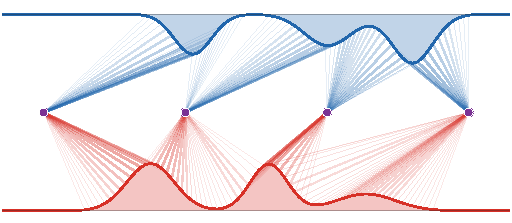
\includegraphics[width=.40\linewidth]{figures/low-rank-ot-factorization/factor-view-r4.pdf} &
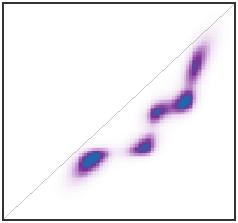
\includegraphics[width=.20\linewidth]{figures/low-rank-ot-factorization/full.pdf} &
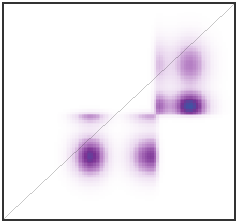
\includegraphics[width=.20\linewidth]{figures/low-rank-ot-factorization/rank-2.pdf}
\\[-.1em]
\small factorization through $r=4$ atoms & \small full entropic plan & \small rank $r=2$
\\[.35em]
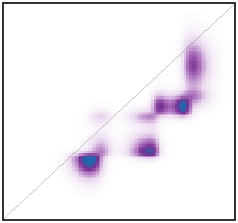
\includegraphics[width=.25\linewidth]{figures/low-rank-ot-factorization/rank-4.pdf} &
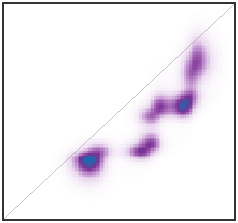
\includegraphics[width=.25\linewidth]{figures/low-rank-ot-factorization/rank-8.pdf} &
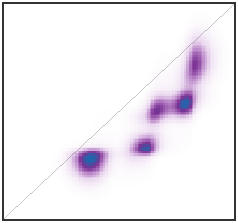
\includegraphics[width=.25\linewidth]{figures/low-rank-ot-factorization/rank-16.pdf}
\\[-.1em]
\small rank $r=4$ & \small rank $r=8$ & \small rank $r=16$
\end{tabular}
\caption{\emph{Low-rank entropic OT on a one-dimensional Gaussian-mixture example with small regularization.} The first panel shows the factorization through an intermediate four-atom measure: red mass couples to violet latent atoms, which then couple to blue mass. The remaining panels compare the full entropic coupling with fixed-latent-mass low-rank couplings of increasing rank. The approximation improves with $r$, but this is deliberately not a favorable example for low rank: in one dimension with a small entropic parameter, quadratic OT is close to a sparse Monge graph rather than to a genuinely low-rank matrix.}
\index{Gaussian!mixture}% strictindex
\index{low-rank!optimal transport}% strictindex
\label{fig:low-rank-ot-factorization}
\end{figure}

\section{Capacity-Constrained Optimal Transport}
\index{capacity-constrained OT}% strictindex
\label{sec-capacity-constrained-ot}

Classical Kantorovich transport only fixes the marginals: if a pair $(x,y)$ is cheap, the optimizer may concentrate as much mass as the marginal constraints allow on this pair. Capacity-constrained OT adds a local congestion rule on the coupling itself. It is useful when edges, facilities or matchings have limited throughput, and it also gives a clean mathematical way to interpolate between a sparse OT plan and the independent product coupling. The systematic study of the continuous problem, including existence and the geometry of active saturated regions, was developed by Korman and McCann~\cite{km1}.
\index{Kantorovich!problem}% strictindex
\index{product!coupling}% strictindex
\index{congestion}% strictindex

Let $\alpha\in\Mm_+^1(\Xx)$, $\beta\in\Mm_+^1(\Yy)$ and let $u:\Xx\times\Yy\to[0,+\infty]$ be a measurable capacity. The capacity-constrained transport value is
\begin{equation}\label{eq-capacity-constrained-ot}
	\MK_c^u(\alpha,\beta)
	\eqdef
	\inf_{\pi\in\Couplings(\alpha,\beta)}
	\enscond{
		\int_{\Xx\times\Yy} c(x,y)\d\pi(x,y)
	}{
		\pi\ll\alpha\otimes\beta,\quad
		\frac{\d\pi}{\d(\alpha\otimes\beta)}(x,y)\leq u(x,y)
	}.
\end{equation}
The product coupling $\alpha\otimes\beta$ is feasible whenever $u\geq1$. Thus the constraint is not meant to promote the product plan; rather, it prevents the optimizer from using any pair more than the prescribed density ratio. Separately, we adopt the convention $\MK_c^{+\infty}(\alpha,\beta)=\MK_c(\alpha,\beta)$: the symbol $u\equiv+\infty$ removes both the density bound and the absolute-continuity requirement, and hence recovers the full Kantorovich problem. At the opposite extreme, $u=1$ forces the independent coupling itself, because a density bounded by one and integrating to one must equal one almost everywhere. Values close to one therefore enforce diffuse plans close to this reference.
\index{density!ratio}% strictindex
\index{product!coupling}% strictindex

For discrete measures $\alpha=\sum_i a_i\de_{x_i}$ and $\beta=\sum_j b_j\de_{y_j}$, a capacity is an upper matrix $\overline{\P}\in\RR_+^{n\times m}$. The density-ratio discretization of~\eqref{eq-capacity-constrained-ot} is $\overline{\P}_{i,j}=u_{i,j}a_i b_j$, and the finite-dimensional problem is the linear program
\index{capacity-constrained OT}% strictindex
\begin{equation}\label{eq-discrete-capacity-constrained-ot}
	\min_{\P\in\CouplingsD(\a,\b)}
	\dotp{\C}{\P}
	\quad\text{subject to}\quad
	0\leq \P_{i,j}\leq \overline{\P}_{i,j}\quad\forall(i,j).
\end{equation}
Feasibility is now a genuine issue: the upper matrix must contain enough mass in every row-column cut to support the prescribed marginals. In particular, the usual transport polytope is recovered when $\overline{\P}_{i,j}=+\infty$, while small capacities select a smaller capped transportation polytope.
\index{upper matrix}% strictindex
\index{capped transportation polytope}% strictindex
\index{transportation polytope}% strictindex
\index{linear!programming}% strictindex

The cut condition can be stated exactly. For index sets $I\subset\{1,\ldots,n\}$ and $J\subset\{1,\ldots,m\}$, write $a(I)=\sum_{i\in I}a_i$, $b(J)=\sum_{j\in J}b_j$, and $\overline{\P}(I,J)=\sum_{i\in I,j\in J}\overline{\P}_{ij}$.

\begin{prop}[Feasibility of a capped transport polytope]\label{prop-capacity-feasibility}
\index{capacity-constrained OT feasibility}% strictindex
	The constraints in~\eqref{eq-discrete-capacity-constrained-ot} are feasible if and only if
	\begin{equation}\label{eq-capacity-cut-condition}
		a(I)+b(J)-1\leq \overline{\P}(I,J)
		\qquad
		\text{for every }I\subset\{1,\ldots,n\},\ J\subset\{1,\ldots,m\}.
	\end{equation}
\end{prop}

\begin{proof}
	If $\P$ is feasible, then
	\[
		\P(I,J)
		=
		a(I)-\P(I,J^c)
		\geq
		a(I)-b(J^c)
		=
		a(I)+b(J)-1.
	\]
	Since $\P(I,J)\leq \overline{\P}(I,J)$, condition~\eqref{eq-capacity-cut-condition} is necessary.

	For sufficiency, build a flow network with capacity $a_i$ from the source to row vertex $i$, capacity $\overline{\P}_{ij}$ from row $i$ to column $j$, and capacity $b_j$ from column $j$ to the sink. A cut containing row set $I$ and column set $J^c$ has capacity
	\[
		1-a(I)+\overline{\P}(I,J)+1-b(J).
	\]
	Condition~\eqref{eq-capacity-cut-condition} says that every such cut has capacity at least one. The max-flow/min-cut theorem therefore gives a unit flow, and its row-to-column edge values form the required matrix $\P$.
\index{max-flow min-cut theorem}% strictindex
\end{proof}

Entropic smoothing gives a direct Sinkhorn-like algorithm. Assume that the cut condition~\eqref{eq-capacity-cut-condition} holds. With $\K_{i,j}=a_i b_j e^{-\C_{i,j}/\epsilon}$, the regularized problem is
\begin{equation}\label{eq-entropic-capacity-constrained-ot}
	\min_{\P\in\CouplingsD(\a,\b),\,0\leq \P\leq \overline{\P}}
	\dotp{\C}{\P}
	+
	\epsilon\KLD(\P|\a\otimes\b).
\end{equation}
Equivalently, up to additive constants, the objective is $\epsilon\KLD(\P|\K)$. The problem is therefore the KL projection of $\K$ onto the intersection of three convex sets: the row constraints, the column constraints and the box $\P\leq \overline{\P}$. Alternating KL projections with Dykstra correction factors~\cite{Dykstra85,bauschke-lewis}, in the same spirit as the Bregman projection formulation of Sinkhorn~\cite{2015-benamou-cisc}, gives a simple capacity-constrained scaling scheme.
\index{entropic!regularization}% strictindex
\index{KL!projection}% strictindex
\index{Bregman!projection}% strictindex
\index{Dykstra algorithm}% strictindex
\index{box constraint}% strictindex

\begin{algH}[Capacity-constrained Sinkhorn by KL-Dykstra]\label{alg-capacity-constrained-sinkhorn}
\index{capacity-constrained Sinkhorn}% strictindex
\textbf{Input:} Positive marginals $\a\in\simplex_n$, $\b\in\simplex_m$, finite cost $\C$, feasible capacity $\overline{\P}$, regularization $\epsilon>0$, tolerance $\mathrm{tol}$.

\textbf{Output:} Entropic capped coupling $\P$.

\textbf{Restrict} all arrays to the active edge set $E=\{(i,j):\overline{\P}_{ij}>0\}$; entries outside $E$ remain zero.

\textbf{Convention:} All products and divisions below are entrywise on $E$.

\textbf{Set} $\K_{i,j}=a_i b_j e^{-\C_{i,j}/\epsilon}$ for $(i,j)\in E$.

\textbf{Initialize:} Set $\P=\K$, correction matrices $R_1=R_2=R_3=\ones_{n\times m}$ and $r=+\infty$.

\textbf{While} $r>\mathrm{tol}$ \textbf{do}:
\begin{algblock}
\textbf{Set} $Z=\P\odot R_1$.

\textbf{Project rows:} $\P= \diag\!\left(\a/(Z\ones_m)\right) Z$.

\textbf{Update} $R_1=Z\oslash \P$.

\textbf{Set} $Z=\P\odot R_2$.

\textbf{Project columns:} $\P= Z\diag\!\left(\b/(Z^\top\ones_n)\right)$.

\textbf{Update} $R_2=Z\oslash \P$.

\textbf{Set} $Z=\P\odot R_3$.

\textbf{Project capacity:} $\P=\min\{Z,\overline{\P}\}$ entrywise.

\textbf{Update} $R_3=Z\oslash \P$.

\textbf{Set} $r=\max\{\|\P\ones_m-\a\|_\infty,\|\P^\top\ones_n-\b\|_\infty,\|(\P-\overline{\P})_+\|_\infty\}$.
\end{algblock}

\textbf{Return} $\P$.
\end{algH}

On the active support, all iterates and correction factors are positive, so every division in Algorithm~\ref{alg-capacity-constrained-sinkhorn} is well defined. KL-Dykstra convergence on finite-dimensional affine and box constraints then shows that, when the capped polytope is nonempty, the iterates converge to the unique minimizer of~\eqref{eq-entropic-capacity-constrained-ot}. Deleting zero-capacity edges before the iteration is essential: writing the correction step directly with a zero cap would create undefined products of zero and infinite correction factors.

\begin{figure}[ht]
\centering
\begin{tabular}{@{}ccc@{}}
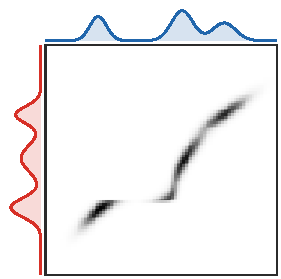
\includegraphics[width=.29\linewidth]{figures/capacity-constrained-ot-1d/large.pdf} &
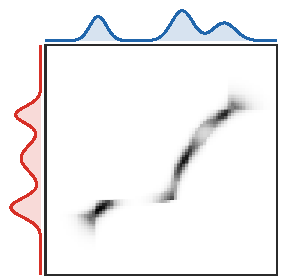
\includegraphics[width=.29\linewidth]{figures/capacity-constrained-ot-1d/medium.pdf} &
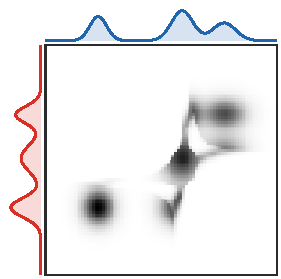
\includegraphics[width=.29\linewidth]{figures/capacity-constrained-ot-1d/small.pdf}
\\[-.1em]
\small unconstrained, $u=+\infty$ &
\small medium capacity, $u=10$ &
\small small capacity, $u=2.6$
\end{tabular}
\caption{\emph{Capacity-constrained entropic OT between two one-dimensional Gaussian-mixture histograms.} Each matrix solves~\eqref{eq-entropic-capacity-constrained-ot} with the same marginals and the same squared-distance cost. The left panel is the unconstrained entropic OT solution, corresponding to the density-ratio cap $\overline{\P}_{ij}=+\infty$. The other panels impose $\overline{\P}_{ij}=u a_i b_j$. The red side strip is the source marginal and the blue top strip is the target marginal. As the capacity decreases, more entries saturate and the coupling is forced to spread.}
\index{Gaussian!mixture}% strictindex
\index{capacity-constrained OT}% strictindex
\label{fig:capacity-constrained-ot-1d}
\end{figure}

For the empirical self-coupling in Figure~\ref{fig:capacity-constrained-ot-2d}, the cap is chosen to prescribe a minimum number of outgoing connections per source point. With uniform weights $a_i=1/n$, imposing $\P_{ij}\leq 1/(qn)$ is equivalent to the conditional bound $\P_{ij}/a_i\leq 1/q$. Since each row has total mass $1/n$, this forces each source row to use at least $q$ target atoms, up to the small extra spreading introduced by entropic smoothing.

\begin{figure}[ht]
\centering
\begin{tabular}{@{}ccc@{}}
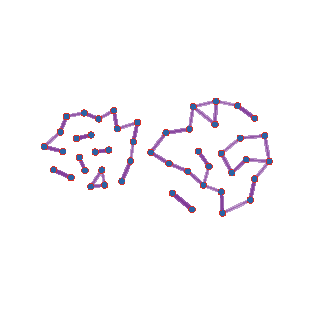
\includegraphics[width=.30\linewidth]{figures/capacity-constrained-ot-2d/cap-1.pdf} &
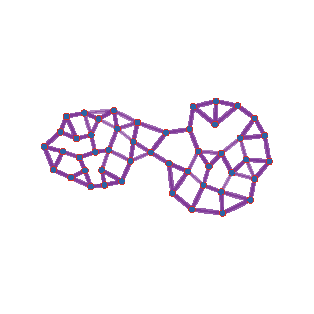
\includegraphics[width=.30\linewidth]{figures/capacity-constrained-ot-2d/cap-3.pdf} &
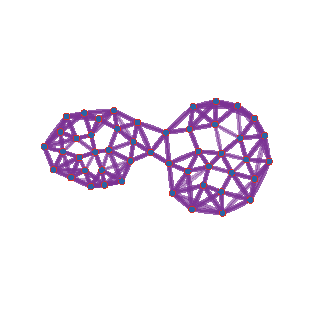
\includegraphics[width=.30\linewidth]{figures/capacity-constrained-ot-2d/cap-5.pdf}
\\[-.1em]
\small one connection, $q=1$ &
\small three connections, $q=3$ &
\small five connections, $q=5$
\end{tabular}
\caption{\emph{Capacity-constrained local self-couplings on a two-dimensional empirical Gaussian mixture.} The source and target are the same semi-regular uniform empirical measure on $n$ atoms, but the diagonal is removed to avoid the trivial identity plan and reveal the local graph selected by the capped problem. Each panel solves~\eqref{eq-entropic-capacity-constrained-ot} with the off-diagonal cap $\overline{\P}_{ij}=1/(qn)$, equivalently $\P_{ij}/a_i\leq 1/q$ since $a_i=1/n$. The three panels therefore impose at least one, three and five outgoing connections per source atom; increasing $q$ forces the local matching to spread over more neighbors.}
\index{empirical!measure}% strictindex
\index{capacity-constrained OT}% strictindex
\label{fig:capacity-constrained-ot-2d}
\end{figure}

\newpage

%%%%%%%%%%%%%%%%%%%%%%%%%%%%%%%%%%%%%%%%%%%%%%%%%%%%%%%%%%%%%%%%%%%%%%%%%%%
%%%%%%%%%%%%%%%%%%%%%%%%%%%%%%%%%%%%%%%%%%%%%%%%%%%%%%%%%%%%%%%%%%%%%%%%%%%
%%%%%%%%%%%%%%%%%%%%%%%%%%%%%%%%%%%%%%%%%%%%%%%%%%%%%%%%%%%%%%%%%%%%%%%%%%%
\section{Metric Learning and Inverse OT}
\label{sec-metric-learning-inverse-ot}
\index{metric!learning}% strictindex
\index{inverse OT}% strictindex

Metric learning differentiates a forward transport loss through a parameterized cost, whereas inverse OT starts from an observed plan and asks which cost makes it optimal. The first viewpoint is often bilevel; the second admits a direct convex formulation for affine cost families, provided the intrinsic cost invariances are removed.
\index{ground cost}% strictindex
\index{bilevel problem}% strictindex
\index{cost!learning}% strictindex

%%%
\subsection{Differentiating OT losses}
\index{metric!learning}% strictindex
\index{cost!derivative}% strictindex
\index{first variation}% strictindex

This subsection records the sensitivity formulas used when the cost or the marginals are learned from data.

\paragraph{First variations of OT values.}
Inverse OT and metric learning repeatedly differentiate a forward OT value with respect to the input law and to the ground cost. The two resulting objects are precisely the two certificates of optimality: a Kantorovich potential for perturbations of the marginal and an optimal coupling for perturbations of the cost. The main caveat is non-uniqueness. In the unregularized case, the correct objects are one-sided directional derivatives, or equivalently subgradients in the measure variable and supergradients in the cost variable. Entropic regularization selects a unique plan and, for positive finite histograms, gives ordinary derivatives on the simplex interiors.
\index{Kantorovich!potential}% strictindex
\index{optimal coupling}% strictindex
\index{directional derivative}% strictindex

\begin{prop}[First variations of unregularized OT]\label{prop-ot-first-variations-unregularized}
	Let $\alpha\in\Pp(\Xx)$ and $\beta\in\Pp(\Yy)$, where $\Xx,\Yy$ are compact metric spaces, and let $c\in\Cc(\Xx\times\Yy)$. Define
	\[
		\mathcal V_c(\alpha,\beta)
		\eqdef
		\inf_{\pi\in\Couplings(\alpha,\beta)}
		\int_{\Xx\times\Yy}c(x,y)\d\pi(x,y).
	\]
	Let $\mathcal O_c(\alpha,\beta)$ be the set of optimal couplings and let $\mathcal D_c(\alpha,\beta)$ be the set of optimal dual potentials $(f,g)$ with $f(x)+g(y)\leq c(x,y)$. If $\chi$ is a signed measure with $\chi(\Xx)=0$ and $\alpha_t=\alpha+t\chi$ is a probability measure for $0\leq t\leq t_0$, then
	\[
		\left.\frac{\d}{\d t}\right|_{t=0^+}
		\mathcal V_c(\alpha_t,\beta)
		=
		\sup_{(f,g)\in\mathcal D_c(\alpha,\beta)}
		\int_{\Xx} f(x)\d\chi(x).
	\]
	If $h\in\Cc(\Xx\times\Yy)$ and $c_t=c+th$, then
	\[
		\left.\frac{\d}{\d t}\right|_{t=0^+}
		\mathcal V_{c_t}(\alpha,\beta)
		=
		\inf_{\pi\in\mathcal O_c(\alpha,\beta)}
		\int_{\Xx\times\Yy} h(x,y)\d\pi(x,y).
	\]
	In particular, if the normalized optimal potential $f^\star$ and the optimal plan $\pi^\star$ are unique, then
	\[
		\frac{\delta \mathcal V_c}{\delta\alpha}=f^\star,
		\qquad
		\frac{\delta \mathcal V_c}{\delta c}=\pi^\star .
	\]
	The second identity means that the first variation with respect to the function $c$ is represented by the optimal measure $\pi^\star$ on $\Xx\times\Yy$.
\index{first variation}% strictindex
\end{prop}
\begin{proof}
	Kantorovich duality writes
	\[
		\mathcal V_c(\alpha,\beta)
		=
		\sup_{f\oplus g\leq c}
		\int f\d\alpha+\int g\d\beta .
	\]
	This is a supremum of affine functions of $\alpha$, so Danskin's theorem gives the one-sided directional derivative as the supremum over active maximizers, namely the optimal dual potentials. The condition $\chi(\Xx)=0$ makes the formula independent of the additive gauge $(f,g)\mapsto(f+\lambda,g-\lambda)$.

	For the cost variable,
	\[
		\mathcal V_{c_t}(\alpha,\beta)
		=
		\inf_{\pi\in\Couplings(\alpha,\beta)}
		\int c\d\pi+t\int h\d\pi
	\]
	is an infimum of affine functions of $t$. Danskin's theorem for a minimum gives the right directional derivative as the infimum of $\int h\d\pi$ over the active minimizers. If the active dual potential or coupling is unique, the corresponding directional derivative is linear in the perturbation, which is the displayed first variation.
\index{first variation}% strictindex
\index{Danskin theorem}% strictindex
\index{envelope theorem}% strictindex
\index{dual!potential}% strictindex
\end{proof}

In the discrete case, this proposition says that any optimal dual vector $f^\star$ is a subgradient with respect to the source weights $\a$, while any optimal plan $\P^\star$ is a supergradient with respect to the cost matrix $\C$, because the value is concave in $\C$:
\[
	f^\star\in\partial_{\a}\MKD_{\C}(\a,\b),
	\qquad
	\P^\star\in\partial_{\C}^{\mathrm{sup}}\MKD_{\C}(\a,\b).
\]
Here $\partial_{\C}^{\mathrm{sup}}$ denotes the superdifferential of the concave map $\C\mapsto\MKD_{\C}(\a,\b)$. When the corresponding objects are unique, these inclusions become the gradients $\nabla_{\a}\MKD_{\C}(\a,\b)=f^\star$ on the tangent space $\{\dotp{\ones}{\chi}=0\}$ and $\nabla_{\C}\MKD_{\C}(\a,\b)=\P^\star$. Without uniqueness, the exact directional derivative with respect to $\C$ in a direction $\Delta\C$ is the minimum of $\dotp{\Delta\C}{\P}$ over all optimal plans.
\index{supergradient}% strictindex
\index{subgradient}% strictindex

\begin{prop}[First variations of entropic OT]\label{prop-ot-first-variations-entropic}
\index{entropic!OT}% strictindex
\index{first variation}% strictindex
	Under the compact-space and continuous-cost assumptions of Proposition~\ref{prop-ot-first-variations-unregularized}, let $\epsilon>0$ and define the KL-normalized entropic value
	\[
		\mathcal V_{c,\epsilon}(\alpha,\beta)
		\eqdef
		\inf_{\pi\in\Couplings(\alpha,\beta)}
		\int c\d\pi+\epsilon\KL(\pi|\alpha\otimes\beta).
	\]
	Choose optimal entropic potentials $(f_\epsilon,g_\epsilon)$ in soft-transform form, so that the following density has marginals $\alpha$ and $\beta$:
	\[
		\d\pi_\epsilon(x,y)
		=
		\exp\pa{\frac{f_\epsilon(x)+g_\epsilon(y)-c(x,y)}{\epsilon}}
		\d\alpha(x)\d\beta(y).
	\]
	This defines the unique optimal coupling. For the same perturbations $\alpha_t=\alpha+t\chi$ and $c_t=c+th$ as in Proposition~\ref{prop-ot-first-variations-unregularized},
	\[
		\left.\frac{\d}{\d t}\right|_{t=0^+}
		\mathcal V_{c,\epsilon}(\alpha_t,\beta)
		=
		\int f_\epsilon\d\chi,
		\qquad
		\left.\frac{\d}{\d t}\right|_{t=0^+}
		\mathcal V_{c_t,\epsilon}(\alpha,\beta)
		=
		\int h\d\pi_\epsilon .
	\]
	Equivalently,
	\[
		\frac{\delta \mathcal V_{c,\epsilon}}{\delta\alpha}=f_\epsilon,
		\qquad
		\frac{\delta \mathcal V_{c,\epsilon}}{\delta c}=\pi_\epsilon .
	\]
	In finite dimension, for positive histograms, these are ordinary derivatives on the relative interior of the simplices.
\end{prop}
\begin{proof}
	The cost derivative follows directly from the primal envelope theorem, because the entropic optimizer is unique. For the measure derivative, use the dual formula~\eqref{eq-dual-sinkhorn-objective}. At an optimal pair, the soft-transform equations imply the row normalization
\index{envelope theorem}% strictindex
	\[
		\int_{\Yy}
		\exp\pa{\frac{f_\epsilon(x)+g_\epsilon(y)-c(x,y)}{\epsilon}}
		\d\beta(y)
		=1
		\qquad\text{for all }x.
	\]
	Differentiating the dual objective with respect to $\alpha$ at fixed optimal potentials gives
	\[
		\int f_\epsilon\d\chi
		-
		\epsilon
		\int_{\Xx\times\Yy}
		\pa{
		e^{(f_\epsilon(x)+g_\epsilon(y)-c(x,y))/\epsilon}-1
		}
		\d\chi(x)\d\beta(y).
	\]
	The second term vanishes by the previous normalization identity, leaving $\int f_\epsilon\d\chi$. The gauge ambiguity of $(f_\epsilon,g_\epsilon)$ again disappears because $\chi(\Xx)=0$.
\index{soft!c-transform}% strictindex
\index{envelope theorem}% strictindex
\end{proof}

For a finite-dimensional parametrization $c_\theta$ or $C_\theta$, the entropic formula gives the backpropagation rule
\[
	\partial_{\theta}\mathcal V_{c_\theta,\epsilon}
	=
	\int \partial_\theta c_\theta(x,y)\d\pi_\epsilon(x,y),
\]
where $\pi_\epsilon$ is the entropic optimizer. For the unregularized value $\mathcal V_{c_\theta}$, uniqueness of the optimal plan $\pi^\star$ gives $\partial_{\theta}\mathcal V_{c_\theta}=\int \partial_\theta c_\theta\d\pi^\star$. Without uniqueness, the directional derivative in a parameter direction $\dot\theta$ is obtained by minimizing $\int \dot\theta\cdot\partial_\theta c_\theta\d\pi$ over the optimal face, while any selected optimal plan gives a valid supergradient with respect to the cost. This is the calculus behind ground-metric learning, which was explicitly studied in~\cite{CuturiGroundMetric2014} and connects to the broader metric-learning literature~\cite{MAL-019,bellet2015metric}. If one uses the entropy-only discrete convention~\eqref{eq-regularized-discr} instead of the KL-normalized value, then, for positive source weights,
\[
	\MKD_\C^\epsilon(\a,\b)
	=
	\mathcal V_{\C,\epsilon}(\a,\b)
	-\epsilon\HD(\a)-\epsilon\HD(\b),
\]
so its derivative with respect to $\a$ is represented on the simplex tangent space by $f_\epsilon+\epsilon\log\a$, up to an irrelevant additive constant.
\index{metric!learning}% strictindex

\begin{figure}[ht]
\centering
\begin{tabular}{@{}ccc@{}}
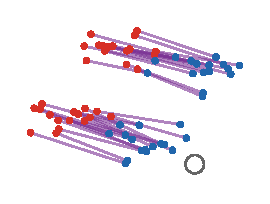
\includegraphics[width=.30\linewidth]{figures/metric-learning-cost-deformation/euclidean.pdf} &
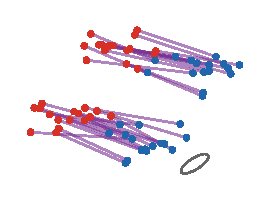
\includegraphics[width=.30\linewidth]{figures/metric-learning-cost-deformation/moderate.pdf} &
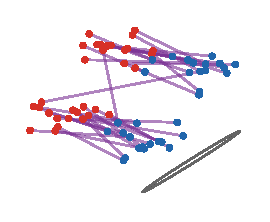
\includegraphics[width=.30\linewidth]{figures/metric-learning-cost-deformation/strong.pdf}
\\[-.1em]
\small Euclidean cost & \small moderate anisotropy & \small strong anisotropy
\end{tabular}
\caption{\emph{Changing the ground metric changes the optimal coupling.} The same red and blue empirical measures are matched with $c_A(x,y)=(x-y)^\top A(x-y)$ for the Euclidean metric and two increasingly anisotropic Mahalanobis metrics. The small gray ellipse shows the unit ball of the metric: directions in which the ellipse is elongated are cheaper, and this deforms the transport segments selected by the OT plan.}
\index{empirical!measure}% strictindex
\label{fig:metric-learning-cost-deformation}
\end{figure}

%%%
\subsection{Inverse Optimal Transport}
\index{inverse OT}% strictindex

Inverse OT asks for a ground cost that explains observed matchings or flows as optimal transport plans. In its most direct form, one observes a plan $\widehat\pi$ with marginals $(\alpha,\beta)$ and seeks a cost $c$ such that $\widehat\pi$ is optimal for
\index{ground cost}% strictindex
\index{plan!transport}% strictindex
\[
	\inf_{\pi\in\Couplings(\alpha,\beta)}\int c(x,y)\d\pi(x,y).
\]
This is ill-posed without structure. Adding $u(x)+v(y)$ to a cost shifts every feasible objective by the same marginal-dependent constant, and multiplying a cost by a positive scalar does not change its minimizers. Moreover, the zero cost rationalizes every feasible plan. An identifiable inverse model must therefore quotient or normalize these gauge and scale freedoms, and a sparse observed plan can still be compatible with a nontrivial cone of normalized costs.
\index{optimal coupling}% strictindex

A useful statistical methodology is to measure the suboptimality of the observed plan through a Fenchel--Young loss. Write the score as $s=-c$ and define the convex regularized prediction value
\index{Fenchel-Young loss}% strictindex
\[
	G_\epsilon(s)=
	\sup_{\pi\in\Couplings(\alpha,\beta)}
	\int s\d\pi-\epsilon\KL(\pi|\alpha\otimes\beta).
\]
The Fenchel--Young loss
\[
	\mathcal L_\epsilon(c;\widehat\pi)
	=
	G_\epsilon(-c)+G_\epsilon^*(\widehat\pi)+\int c\d\widehat\pi
\]
is nonnegative by Fenchel's inequality and vanishes exactly when $\widehat\pi\in\partial G_\epsilon(-c)$, i.e. when $\widehat\pi$ satisfies the regularized optimality conditions for $c$. Sharpened Fenchel--Young losses for inverse problems over measures and inverse entropic/unbalanced OT are developed in~\cite{andrade2025sharpened}; curvature and identifiability of inverse OT with respect to the cost are studied in~\cite{peyre2026curvature}. Entropic regularization is important here because it makes the forward map smoother and provides gradients with respect to $c$, at the price of a bias that must be controlled statistically.
\index{Fenchel-Young loss}% strictindex
\index{entropic!regularization}% strictindex
\index{unbalanced!OT}% strictindex

In the discrete unregularized case, this loss reduces to the optimality gap of the observed coupling. For $\widehat P\in\CouplingsD(\a,\b)$ and a cost matrix $C$, denote it by
\[
	\mathcal L_{\mathrm{iOT}}(C;\widehat P)
	=
	\dotp{C}{\widehat P}
	-
	\umin{P\in\CouplingsD(\a,\b)} \dotp{C}{P}.
\]
This inverse-OT gap loss is nonnegative and vanishes exactly when $\widehat P$ is optimal for $C$.
\index{inverse OT gap loss}% strictindex

In practice, one restricts the cost to a finite-dimensional model class, often affine:
\[
	C_\theta=\sum_{r=1}^R \theta_r C^{(r)},
	\qquad \theta\in\Theta,
\]
where $\Theta$ is convex and the matrices $C^{(r)}$ encode features, graph distances or a Mahalanobis parameterization. This viewpoint appears in low-rank and sparse inverse OT models~\cite{dupuy2016estimating,andrade2024sparsistency} and in convex formulations for learning OT costs from observed plans~\cite{ma2020learning,peyre2026curvature}.

\index{inverse OT}% strictindex
A minimal finite-dimensional model is obtained by learning a bilinear cost on $\RR^d$,
\[
	c_A(x,y)=\dotp{Ax}{y},
	\qquad A\in\RR^{d\times d}.
\]
For empirical measures $\al=\frac1n\sum_i\de_{x_i}$ and $\be=\frac1n\sum_j\de_{y_j}$, this gives the cost matrix
\[
	C(A)_{i,j}=\dotp{Ax_i}{y_j},
\]
so both maps $A\mapsto C(A)$ and $A\mapsto c_A$ are linear. Inverse OT within this model asks which matrix $A$ makes an observed matching or coupling look optimal; learning the cost is thus reduced to estimating a linear parameter.
\index{bilinear cost}% strictindex

For a fixed matrix $A$, the forward prediction is the optimal face
\[
	\mathcal P_A\eqdef
	\uargmin{P\in\CouplingsD(\ones_n/n,\ones_n/n)}
	\dotp{C(A)}{P}.
\]
When this face is a singleton, write its element as $P_A$; otherwise $P_A$ denotes a deterministic tie-broken selection. Although $A\mapsto C(A)$ is linear, the solution correspondence $A\mapsto\mathcal P_A$ is polyhedral: changing $A$ changes the direction in which the transport polytope is probed, and a tie-broken selection is constant on normal-cone cells. Figure~\ref{fig:inverse-ot-forward-logo} illustrates this correspondence on the OT4ML point clouds. The construction follows the visual idea of the Python Optimal Transport logo~\cite{flamary2021pot}: red source atoms, blue target atoms and straight segments show the selected optimal bijection. With $e=(1,1)^\top$ and $\delta=10^{-3}$, the first two rank-one matrices are $A_h=-e_1e^\top+\delta e_2e^\top$ and $A_v=\delta e_1e^\top-e_2e^\top$. These small transverse terms break the large ties of the pure horizontal or vertical scores while preserving a rank-one cost. The matrix $A=-\Id$ gives the usual quadratic $\Wass_2$ assignment, up to the marginal-only terms discussed below, while $A=+\Id$ reverses the correlation and produces an anti-$\Wass_2$ matching.

\begin{figure}[ht]
\centering
\begin{tabular}{@{}cc@{}}
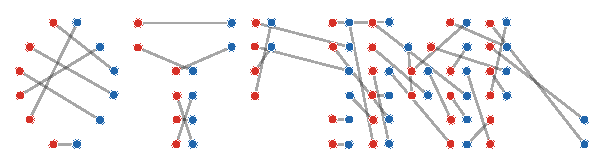
\includegraphics[width=.48\linewidth]{figures/inverse-ot-bilinear-logo-map/horizontal.pdf} &
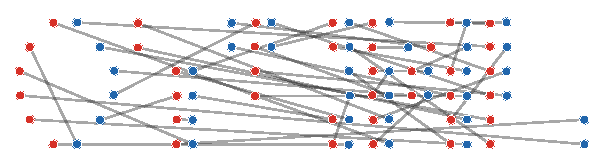
\includegraphics[width=.48\linewidth]{figures/inverse-ot-bilinear-logo-map/vertical.pdf}
\\[-.1em]
\small horizontal, $A_h=(-e_1+\delta e_2)e^\top$ &
\small vertical, $A_v=(\delta e_1-e_2)e^\top$
\\[.35em]

\includegraphics[width=.48\linewidth]{figures/inverse-ot-bilinear-logo-map/w2.pdf} &
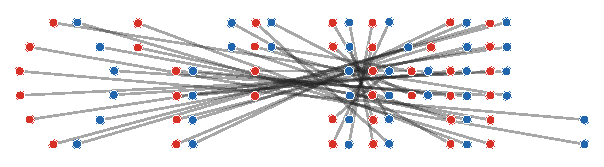
\includegraphics[width=.48\linewidth]{figures/inverse-ot-bilinear-logo-map/anti.pdf}
\\[-.1em]
\small quadratic $\Wass_2$, $A=-\Id$ &
\small anti-$\Wass_2$, $A=+\Id$
\end{tabular}
\caption{\emph{Forward solutions of the bilinear cost $c_A(x,y)=\dotp{Ax}{y}$ on the OT4ML logo point clouds.} Each panel solves the equal-weight assignment problem with a different matrix $A$; the first two use $\delta=10^{-3}$ to break rank-one ties. The source atoms are red, the target atoms are blue, and the gray segments give one deterministic optimal bijection.}
\label{fig:inverse-ot-forward-logo}
\end{figure}

This elementary model already contains the quadratic Wasserstein assignment. Adding to a cost matrix a term depending only on $x_i$ or only on $y_j$ shifts all feasible couplings by the same constant, and therefore does not change the optimizer. Since
\[
	\norm{x-y}^2=\norm{x}^2+\norm{y}^2-2\dotp{x}{y},
\]
the usual quadratic Wasserstein assignment has the same optimizer as the bilinear cost with $A_\star=-\Id$, up to these marginal-only terms and an irrelevant positive factor. The inverse problem goes in the opposite direction: after observing a coupling, one asks which matrices $A$ could have generated it. Figure~\ref{fig:inverse-ot-gap-loss} generates an observed coupling $\widehat P$ from this cost on two empirical mixtures of Gaussians, and then evaluates $\mathcal L_{\mathrm{iOT}}(C(A_t);\widehat P)$ along the anisotropic path
\[
	A_t=-\diag(1+t,1-t),
	\qquad -1\leq t\leq 1,
\]
so that $t=0$ recovers the matrix that generated the observed coupling. Equivalently, with equal weights, $\widehat P\in\CouplingsD(\ones_n/n,\ones_n/n)=\mathcal B_n/n$ and the plotted loss is the Kantorovich gap
\[
	\mathcal L_{\mathrm{iOT}}(C(A_t);\widehat P)
	=
	\dotp{C(A_t)}{\widehat P}
	-
	\umin{P\in\CouplingsD(\ones_n/n,\ones_n/n)}
	\dotp{C(A_t)}{P},
	\qquad
	C(A_t)_{i,j}=\dotp{A_t x_i}{y_j}.
\]
Because $t\mapsto C(A_t)$ is affine and the Kantorovich value is a minimum of affine functions over the fixed polytope $\CouplingsD(\ones_n/n,\ones_n/n)$, this one-dimensional gap is convex and piecewise affine. Its zero set can contain an interval for a small sample, reflecting the fact that the same observed coupling remains optimal for a cone of nearby costs.

\begin{figure}[ht]
\centering
\begin{tabular}{@{}ccc@{}}
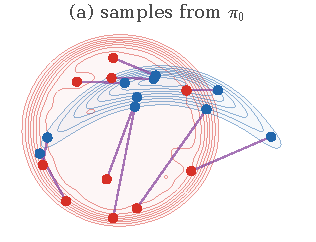
\includegraphics[width=.35\linewidth]{figures/inverse-ot-gap-loss/observed-map-n10.pdf} &
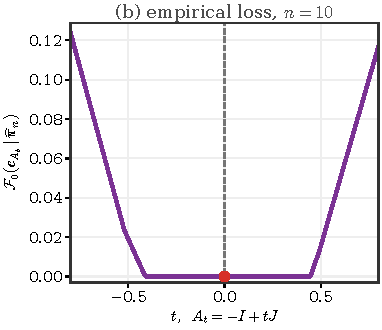
\includegraphics[width=.29\linewidth]{figures/inverse-ot-gap-loss/gap-loss-n10.pdf} &
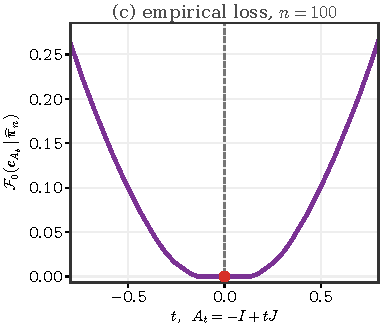
\includegraphics[width=.29\linewidth]{figures/inverse-ot-gap-loss/gap-loss-n100.pdf}
\\[-.1em]
\small observed map, $n=10$ &
\small loss curve, $n=10$ &
\small loss curve, $n=100$
\end{tabular}
\caption{\emph{Inverse-OT gap loss for a bilinear cost.} Panel (a): two empirical mixtures of two Gaussians are matched with the cost $c_{A_\star}(x,y)=\dotp{A_\star x}{y}$ for $A_\star=-\Id$, which gives the same optimizer as the quadratic $\Wass_2$ cost; red and blue level sets display the two sampling densities. Panels (b,c): the unregularized Fenchel--Young Kantorovich gap $\mathcal L_{\mathrm{iOT}}(C(A_t);\widehat P)$ along $A_t=-\diag(1+t,1-t)$ for $n=10$ and $n=100$, using the same vertical scale. The red dot marks the generating parameter $t=0$; the curves are convex and piecewise affine.}
\label{fig:inverse-ot-gap-loss}
\end{figure}

The comparison between $n=10$ and $n=100$ illustrates an important statistical effect: as the number of sampled points grows, the flat zero region can shrink to a sharper piecewise-affine minimum. A finite-sample linear-programming gap remains polyhedral and therefore has no classical second derivative inside its cells. Curvature is instead a population phenomenon. Peyr\'e, Poon and Tron~\cite{peyre2026curvature} prove local curvature and identifiability modulo the natural cost invariances for smooth positive marginals under a nondegeneracy condition. They also identify affine-map settings, including Gaussian or elliptical examples, as genuinely degenerate cases. Thus larger samples can reveal population curvature, but do not remove structural non-identifiability by themselves.

\begin{prop}[Convex dual-gap formulation of inverse OT]\label{prop-inverse-ot-convex}
\index{dual!gap}% strictindex
\index{inverse OT}% strictindex
	Let $\widehat P\in\CouplingsD(\a,\b)$ be an observed coupling and let $C_\theta$ depend affinely on $\theta\in\Theta$, where $\Theta$ is convex. The condition that $\widehat P$ is optimal for the cost $C_\theta$ is equivalent to the existence of dual potentials $(f,g)$ such that
\index{dual!potential}% strictindex
	\[
		f_i+g_j\leq (C_\theta)_{i,j}
		\qandq
		\sum_{i,j}\widehat P_{i,j}\big((C_\theta)_{i,j}-f_i-g_j\big)=0.
	\]
	Consequently, for a convex regularizer $R$ and $\lambda\geq0$, the dual-gap fitting problem
\index{convex!regularizer}% strictindex
	\eql{\label{eq-inverse-ot-convex}
		\umin{\theta\in\Theta,f,g}
		R(\theta)+\lambda
		\sum_{i,j}\widehat P_{i,j}\big((C_\theta)_{i,j}-f_i-g_j\big)
		\quad\text{subject to}\quad
		f_i+g_j\leq (C_\theta)_{i,j}\quad\forall i,j.
	}
	is convex. It is nontrivial only if $\Theta$ imposes a cost normalization or otherwise excludes the zero-cost and marginal-gauge degeneracies.
\end{prop}

\begin{proof}
	For a fixed cost $C_\theta$, Kantorovich duality gives
\index{Kantorovich!duality}% strictindex
	\[
		\min_{P\in\CouplingsD(\a,\b)}\dotp{C_\theta}{P}
		=
		\max_{f_i+g_j\leq (C_\theta)_{i,j}}
		\dotp{f}{\a}+\dotp{g}{\b}.
	\]
	Since $\widehat P$ has marginals $(\a,\b)$, every dual feasible pair satisfies
	\[
		\dotp{C_\theta}{\widehat P}-\dotp{f}{\a}-\dotp{g}{\b}
		=
		\sum_{i,j}\widehat P_{i,j}\big((C_\theta)_{i,j}-f_i-g_j\big)
		\geq0.
	\]
	This nonnegative quantity is exactly the primal-dual gap of $\widehat P$. It vanishes if and only if $\widehat P$ reaches the dual value and is therefore optimal. If $C_\theta$ is affine, $\lambda\geq0$, and $\Theta$ and $R$ are convex, the constraints and objective in~\eqref{eq-inverse-ot-convex} are convex. If $C_\theta=0$ is allowed and minimizes $R$, then $(C,f,g)=(0,0,0)$ is a trivial minimizer; this proves the need for the normalization stated above.
\index{dual!gap}% strictindex
\end{proof}

\begin{alg}[Inverse OT by dual-gap fitting]\label{alg:inverse-ot-dual-gap-learning}
\index{inverse OT}% strictindex
\textbf{Input:} Observed plan $\widehat P\in\CouplingsD(\a,\b)$, features $C^{(r)}$, normalized convex feasible set $\Theta$, convex regularizer $R$, weight $\lambda>0$.

\textbf{Output:} Identified cost $C_{\theta^\star}$ and potentials $(f^\star,g^\star)$.

\textbf{Set} parametric cost:
\(C_\theta=\sum_r\theta_r C^{(r)}.\)

\textbf{Let} $(\theta^\star,f^\star,g^\star)$ be a minimizer of
\(\min_{\theta\in\Theta,f,g} R(\theta)+\lambda \sum_{i,j}\widehat P_{i,j}\big((C_\theta)_{i,j}-f_i-g_j\big)\)

\textbf{Subject to}
\(f_i+g_j\leq(C_\theta)_{i,j} \qquad\text{for all }(i,j).\)
\textbf{Return} $\theta^\star$, $C_{\theta^\star}$, and $(f^\star,g^\star)$.
\end{alg}

The formulation~\eqref{eq-inverse-ot-convex} avoids differentiating through a forward OT solver: it learns a normalized cost by making the observed plan nearly satisfy complementary slackness. In statistical settings, $\widehat P$ is only partially observed or noisy, so one adds sparsity, low-rank, smoothness or metric constraints to select a meaningful representative~\cite{dupuy2016estimating,andrade2024sparsistency}. For entropic OT, the optimality condition becomes smoother:
\index{entropic!OT}% strictindex
\index{complementary slackness}% strictindex
\[
	\widehat P_{i,j}\approx a_i b_j
	\exp\pa{\frac{f_i+g_j-(C_\theta)_{i,j}}{\epsilon}},
\]
which leads to likelihood-based or KL-based convex objectives when $C_\theta$ is affine, and connects inverse OT with generalized Sinkhorn iterations and transport-regularized inverse problems~\cite{karlsson2016generalized,ma2020learning}. Neural parameterizations of $C_\theta$ are more flexible but reintroduce non-convexity; the convex formulation above is the clean mathematical baseline.
\index{Sinkhorn!iteration}% strictindex


%%%%%%%%%%%%%%%%%%%%%%%%%%%%%%%%%%%%%%%%%%%%%%%%%%%%%%%%%%%%%%%%%%%%%%%%%%%


%%%%%%%%%%%%%%%%%%%%%%%%%%%%%%%%%%%%%%%%%%%%%%%%%%%%%%%%%%%%%%%%%%%%%%%%%%%
%%%%%%%%%%%%%%%%%%%%%%%%%%%%%%%%%%%%%%%%%%%%%%%%%%%%%%%%%%%%%%%%%%%%%%%%%%%
%%%%%%%%%%%%%%%%%%%%%%%%%%%%%%%%%%%%%%%%%%%%%%%%%%%%%%%%%%%%%%%%%%%%%%%%%%%
\section{Weak Optimal Transport}
\index{weak!optimal transport}% strictindex
\label{sec-weak-ot}

Weak OT relaxes the cost so that it depends on the conditional distribution of destinations rather than only on pointwise pairs. It is useful when a source point is allowed to choose a randomized response and the model only penalizes an aggregate of that response, such as its conditional mean.
\index{conditional!law}% strictindex

\paragraph{Barycentric projection of a coupling.}
\index{barycentric!projection}% strictindex
The first object to isolate is therefore the map obtained by collapsing each conditional law to its barycenter.

\begin{defn}[Barycentric projection of a coupling]\label{def-barycentric-projection}
	Let $\alpha,\beta\in\Pp_1(\RR^d)$ and let $\pi\in\Couplings(\alpha,\beta)$. Disintegrate $\pi$ with respect to its first marginal as
	$\pi(\d x,\d y)=\pi_x(\d y)\alpha(\d x)$. Since $\beta$ has finite first moment, the conditional mean is finite for $\alpha$-a.e. $x$, and the barycentric projection of $\pi$ is the map
	\begin{equation}\label{eq-barycentric-projection}
		\bar T_\pi(x)
		\eqdef
		\int_{\RR^d}y\d\pi_x(y),
		\qquad
		\bar\beta_\pi
		\eqdef
		(\bar T_\pi)_\sharp\alpha.
	\end{equation}
\end{defn}
The projected target $\bar\beta_\pi$ records the distribution of conditional means, not the full second marginal. Thus it is generally different from $\beta$; if $\pi=(\Id,T)_\sharp\alpha$ is induced by a map, then $\bar T_\pi=T$ and $\bar\beta_\pi=\beta$. This projection is not an optimal map for an arbitrary coupling: a deterministic rotation of a radially symmetric source, for example, projects to the rotation itself, whereas the optimal map from the source to itself is the identity. The useful positive statement is attached to quadratic optimal plans, as in the tangent-space viewpoint on $\Wass_2$ developed by Ambrosio, Gigli and Savar{\'e}~\cite[Chap.~7]{ambrosio2006gradient}.
\index{optimal plan}% strictindex

\begin{prop}[Barycentric projection of a quadratic optimal plan]\label{prop-barycentric-projection-optimal}
\index{barycentric!projection}% strictindex
	Let $\pi\in\Couplings(\alpha,\beta)$ be optimal for the quadratic cost $\norm{x-y}^2$ between $\alpha,\beta\in\Pp_2(\RR^d)$, and define $\bar T_\pi$ and $\bar\beta_\pi$ by~\eqref{eq-barycentric-projection}. Then $(\Id,\bar T_\pi)_\sharp\alpha$ is an optimal coupling between $\alpha$ and $\bar\beta_\pi$. Equivalently, $\bar T_\pi$ is a quadratic optimal transport map from $\alpha$ to the projected target $\bar\beta_\pi$.
\index{optimal coupling}% strictindex
\index{transport!map}% strictindex
\index{quadratic!cost}% strictindex
\end{prop}

\begin{proof}
	By Theorem~\ref{thm:opt_ccm}, $\pi$ is concentrated on a $c$-cyclically monotone set $\Gamma$ for $c(x,y)=\norm{x-y}^2$. For the quadratic cost, and since it is enough to check cyclic permutations, this means that every finite cycle $(x_i,y_i)_{i=1}^m\subset\Gamma$ satisfies
	\[
		\sum_{i=1}^m \dotp{x_i}{y_i}
		\geq
		\sum_{i=1}^m \dotp{x_i}{y_{i+1}},
		\qquad y_{m+1}=y_1.
	\]
	After changing the disintegration on an $\alpha$-negligible set, $\pi_x$ is supported on the section
\index{disintegration}% strictindex
	\[
		\Gamma_x=\enscond{y}{(x,y)\in\Gamma}
	\]
	for $\alpha$-a.e. $x$.
	Choose $x_1,\ldots,x_m$ in this full-measure set and independently sample $Y_i\sim\pi_{x_i}$. Applying the cyclic inequality to $(x_i,Y_i)$ and taking expectations gives
	\[
		\sum_{i=1}^m \dotp{x_i}{\bar T_\pi(x_i)}
		\geq
		\sum_{i=1}^m \dotp{x_i}{\bar T_\pi(x_{i+1})}.
	\]
	Thus $(\Id,\bar T_\pi)_\sharp\alpha$ is concentrated on a cyclically monotone graph. By the cyclic-monotonicity characterization of quadratic optimality, this plan is optimal between its two marginals, namely $\alpha$ and $\bar\beta_\pi$.
\index{cyclic!monotonicity}% strictindex
\end{proof}

\begin{rem}[Barycentric projection appears everywhere]\label{rem-barycentric-projection-everywhere}
\index{barycentric!projection}% strictindex
\index{conditional!mean}% strictindex
	Barycentric projection is the operation that turns a conditional law into a mean. Definition~\ref{def-barycentric-projection} and \eqref{eq-barycentric-projection} apply this to a coupling disintegrated as \(\pi(\d x,\d y)=\pi_x(\d y)\alpha(\d x)\), and Proposition~\ref{prop-barycentric-projection-optimal} shows that quadratic optimal plans are stable under this collapse. The same operation is the organizing summary in weak OT: the barycentric weak cost in Proposition~\ref{prop-barycentric-weak-ot} is obtained by inserting \(\bar T_\pi\) into \eqref{eq-weak-ot}. Martingale OT fixes this summary instead of merely penalizing it, imposing \(\int y\,\d\pi_x(y)=x\) in \eqref{eq-martingale-coupling}. Conditional Wasserstein distances in Definition~\ref{def-conditional-ot} use the same disintegration language fiber by fiber, see \eqref{eq-conditional-ot-general}. Later, the mean-shift and Gaussian-attention velocity \eqref{eq-l2-attention-mean-shift} is again a barycentric average, now of a kernel-weighted neighborhood, and SVGD in Section~\ref{sec-svgd-generative-flow} replaces this barycentric averaging by the RKHS steepest-descent average \eqref{eq-svgd-velocity}. Across these examples, the recurring move is to keep the conditional structure of a coupling but replace the full conditional law by a tractable first moment or kernelized moment.
\end{rem}

\paragraph{Weak transport costs.}
\index{weak!optimal transport}% strictindex
\index{weak!C-transform}% strictindex
Weak transport costs use the same disintegration but allow the objective to depend on the whole conditional law, or on summaries such as the barycentric projection~\eqref{eq-barycentric-projection}. The framework was introduced through general transport costs and weak transport inequalities in~\cite{gozlan2017kantorovich}; existence, duality and optimality conditions on Polish spaces are developed in~\cite{backhoff2019weak}. For a weak cost $C:\Xx\times\Pp(\Yy)\to\RR\cup\{+\infty\}$, the weak OT value is
\index{weak!cost}% strictindex
\index{disintegration}% strictindex
\index{conditional!law}% strictindex
\index{barycentric!projection}% strictindex
\index{weak!transport}% strictindex
\index{Polish space}% strictindex
\begin{equation}\label{eq-weak-ot}
	\WOT_C(\alpha,\beta)
	\eqdef
	\inf_{\pi\in\Couplings(\alpha,\beta)}
	\int C(x,\pi_x)\d\alpha(x).
\end{equation}
The classical Kantorovich problem is recovered when $C(x,\nu)=\int c(x,y)\d\nu(y)$, because the objective then becomes $\int c(x,y)\d\pi(x,y)$. The genuinely weak behavior starts when $C$ is nonlinear in $\nu$.
\index{Kantorovich!problem}% strictindex

\begin{prop}[Weak Kantorovich duality]\label{prop-weak-ot-duality}
\index{Kantorovich!duality}% strictindex
\index{weak!Kantorovich duality}% strictindex
	Let $\Xx$ and $\Yy$ be compact metric spaces, and let $C:\Xx\times\Pp(\Yy)\to\RR\cup\{+\infty\}$ be proper, jointly lower semicontinuous, bounded from below and convex in its second argument. Fix $\alpha\in\Pp(\Xx)$ and $\beta\in\Pp(\Yy)$, and assume that $\WOT_C(\alpha,\beta)<+\infty$. For $g\in\Cc(\Yy)$, define the weak $C$-transform
\index{duality!Fenchel-Rockafellar}% strictindex
\index{lower semicontinuity}% strictindex
\index{Fenchel duality}% strictindex
	\[
		g^C(x)
		\eqdef
		\inf_{\nu\in\Pp(\Yy)}
		\left\{
			C(x,\nu)-\int g(y)\d\nu(y)
		\right\}.
	\]
	Then
	\[
		\WOT_C(\alpha,\beta)
		=
		\sup_{g\in\Cc(\Yy)}
		\left\{
			\int g^C(x)\d\alpha(x)+\int g(y)\d\beta(y)
		\right\}.
	\]
	When $C(x,\nu)=\int c(x,y)\d\nu(y)$, this reduces to the usual Kantorovich dual with $g^C(x)=\inf_y(c(x,y)-g(y))$.
\end{prop}

\begin{proof}
	For any coupling $\pi$ and any $g\in\Cc(\Yy)$, the definition of $g^C$ gives
	\[
		C(x,\pi_x)\geq g^C(x)+\int g(y)\d\pi_x(y).
	\]
	After integration with respect to $\alpha$, the second term becomes $\int g\d\beta$ because the second marginal of $\pi$ is $\beta$. This proves weak duality.
\index{duality!weak}% strictindex

	For the converse, lift a kernel $x\mapsto\pi_x$ to the measure $\alpha(\d x)\delta_{\pi_x}(\d\nu)$ on $\Xx\times\Pp(\Yy)$. Relaxing this graph constraint gives probability measures $P$ whose first marginal is $\alpha$ and whose intensity satisfies
	\[
		\int_{\Xx\times\Pp(\Yy)}\nu\,\d P(x,\nu)=\beta.
	\]
	This relaxation does not change the value: disintegrating $P(\d x,\d\nu)=P_x(\d\nu)\alpha(\d x)$ and replacing $P_x$ by its barycenter $\bar\nu_x=\int\nu\,\d P_x(\nu)$ preserves the intensity constraint and cannot increase the objective, by convexity of $C(x,\cdot)$. The relaxed feasible set is compact, and the integral functional is lower semicontinuous. Fenchel--Rockafellar duality for the affine intensity constraint therefore has no gap; its continuous multiplier is $g\in\Cc(\Yy)$. Minimization in $\nu$ gives $g^C(x)$, while the constraint contributes $\int g\d\beta$. This is the weak-cost analogue of Proposition~\ref{prop-duality-discr}; see~\cite{backhoff2019weak} for the Polish-space formulation.
\index{duality!Fenchel-Rockafellar}% strictindex
\index{lower semicontinuity}% strictindex
\index{Fenchel duality}% strictindex
\index{conditional!law}% strictindex
\index{marginal!constraint}% strictindex
\index{affine!constraint}% strictindex
\end{proof}

\begin{prop}[Barycentric weak transport is weaker than $\Wass_2$]\label{prop-barycentric-weak-ot}
\index{weak!transport}% strictindex
	Let $\alpha,\beta\in\Pp_2(\RR^d)$ and define
	\[
		C_{\mathrm{bar}}(x,\nu)
		=
		\norm{x-\int y\d\nu(y)}^2.
	\]
	Equivalently, for a coupling $\pi$, the integrand is $\norm{x-\bar T_\pi(x)}^2$. Then
	\[
		\WOT_{C_{\mathrm{bar}}}(\alpha,\beta)
		\leq
		\Wass_2^2(\alpha,\beta).
	\]
\end{prop}

\begin{proof}
	Let $\pi$ be any coupling and disintegrate it as $\pi_x\alpha$. By Jensen's inequality,
\index{Jensen inequality}% strictindex
\index{disintegration}% strictindex
	\[
		\norm{x-\bar T_\pi(x)}^2
		\leq
		\int\norm{x-y}^2\d\pi_x(y).
	\]
	Integrating in $x$ gives $\int C_{\mathrm{bar}}(x,\pi_x)\d\alpha(x)\leq\int\norm{x-y}^2\d\pi(x,y)$. Taking the infimum over $\pi$ proves the claim.
\end{proof}

\begin{figure}[H]
\centering
\begin{tabular}{@{}cc@{}}
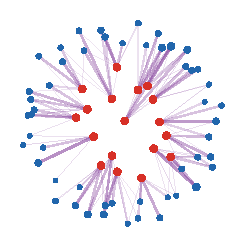
\includegraphics[width=.43\linewidth]{figures/weak-ot-barycentric-projection/conditional-coupling.pdf} &
\index{barycentric!projection}% strictindex
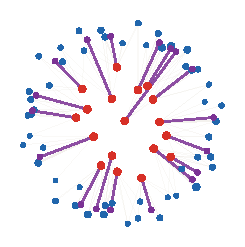
\includegraphics[width=.43\linewidth]{figures/weak-ot-barycentric-projection/barycentric-projection.pdf}
\\[-.1em]
\small conditionals $\pi_x$ & \small barycentric projection $\bar T_\pi$
\end{tabular}
\caption{\emph{Weak barycentric transport on a small disk-to-annulus coupling.} The left panel shows the full conditional laws: each red source atom splits its mass among several blue target atoms, with segment thickness proportional to transported mass. The right panel collapses each conditional law $\pi_x$ to its barycenter $\bar T_\pi(x)=\int y\d\pi_x(y)$, shown in violet. The barycentric weak cost only sees the red-to-violet displacement, and therefore ignores the conditional spread around each barycenter.}
\index{weak!cost}% strictindex
\index{barycentric!transport}% strictindex
\label{fig:weak-ot-barycentric-projection}
\end{figure}

\index{conditional!variance}% strictindex
\index{barycentric!constraint}% strictindex
The barycentric cost is the canonical example to keep in mind: admissibility still constrains the full conditional laws to have second marginal $\beta$, but the objective only charges the displacement from $x$ to $\bar T_\pi(x)$ and ignores the conditional variance around this barycenter. This connects weak OT with martingale transport, Strassen-type convex-order constraints, barycentric projections and learning problems where conditional averages are meaningful objects.
\index{conditional!law}% strictindex
\index{barycentric!projection}% strictindex

\subsection{Martingale Optimal Transport}
\index{mean-preserving splitting}% strictindex
\index{robust!finance}% strictindex
\index{martingale OT}% strictindex
\label{sec-martingale-ot}

Martingale OT is the extreme barycentric version of the weak viewpoint: a source point may split randomly, but the average destination must remain equal to the source point. This turns the barycentric projection from an object used in the cost into a hard constraint.

\begin{defn}[Martingale couplings and martingale OT]\label{def-martingale-coupling}
\index{martingale coupling}% strictindex
	Let $\alpha,\beta\in\Pp_1(\RR^d)$. A coupling $\pi\in\Couplings(\alpha,\beta)$ is a martingale coupling if, for the disintegration $\pi(\d x,\d y)=\pi_x(\d y)\alpha(\d x)$,
	\begin{equation}\label{eq-martingale-coupling}
		\int_{\RR^d}y\d\pi_x(y)=x
		\qquad\text{for $\alpha$-a.e. }x .
	\end{equation}
	Equivalently, $\bar T_\pi=\Id$ in~\eqref{eq-barycentric-projection}. The set of such couplings is denoted
	\[
		\Couplings_{\mathrm{mart}}(\alpha,\beta)
		\eqdef
		\enscond{\pi\in\Couplings(\alpha,\beta)}{\bar T_\pi=\Id\quad\alpha\text{-a.e.}}.
	\]
\end{defn}

For a cost $c$, the martingale OT problem minimizes $\int c\d\pi$ over $\Couplings_{\mathrm{mart}}(\alpha,\beta)$, with value $+\infty$ when the admissible set is empty.
\index{martingale OT}% strictindex

The terminology comes from probability: if $(X,Y)\sim\pi$, then~\eqref{eq-martingale-coupling} is exactly $\EE[Y|X]=X$. Hence martingale OT is a Kantorovich problem with the usual two marginal constraints plus a barycentric constraint on the conditional laws. Equivalently, the barycentric projected coupling
\[
	(\Id,\bar T_\pi)_\sharp\alpha
\]
must be the diagonal coupling $(\Id,\Id)_\sharp\alpha$. This is stronger than merely asking the projected target $(\bar T_\pi)_\sharp\alpha$ to equal $\alpha$, since a nontrivial measure-preserving map could have the same projected marginal without satisfying $\bar T_\pi(x)=x$ pointwise. Martingale OT is central in robust finance, where one transports today prices to tomorrow prices without introducing drift, and has led to a rich martingale transport theory~\cite{beiglbock2013model,GalichonMartingale,dolinsky2014martingale,guo2017computational}.
\index{conditional!expectation}% strictindex
\index{marginal!constraint}% strictindex
\index{diagonal coupling}% strictindex

\paragraph{Stochastic orders.}
\index{stochastic!order}% strictindex
The admissibility of constrained couplings is governed by stochastic order. The basic principle is that inequalities tested against a class of functions are equivalent to the existence of couplings satisfying a pointwise or conditional constraint. Strassen's theorem is the canonical result of this kind~\cite{Strassen1965}.
\index{martingale coupling}% strictindex
\index{Strassen theorem}% strictindex
\index{order-constrained coupling}% strictindex

\begin{prop}[Strassen's theorem for stochastic order]\label{prop-strassen-stochastic-order}
\index{stochastic!order}% strictindex
	Let $\alpha,\beta\in\Pp(\RR)$ and define the classical stochastic order by
	\[
		\alpha\preceq_{\mathrm{st}}\beta
		\quad\Longleftrightarrow\quad
		\int \varphi\,\d\alpha\leq\int \varphi\,\d\beta
		\quad\text{for every bounded increasing }\varphi .
	\]
	Then $\alpha\preceq_{\mathrm{st}}\beta$ if and only if there exists $\pi\in\Couplings(\alpha,\beta)$ concentrated on $\enscond{(x,y)}{x\leq y}$.
\end{prop}

\begin{proof}
	A coupling supported on $x\leq y$ immediately gives the integral inequality for every increasing $\varphi$. Conversely, testing approximate indicators of intervals $(t,+\infty)$ gives $F_\alpha(t)\geq F_\beta(t)$ for all continuity points of the distribution functions. If $U$ is uniform on $(0,1)$ and $F_\alpha^{-1},F_\beta^{-1}$ are the generalized quantiles, then $X=F_\alpha^{-1}(U)$ and $Y=F_\beta^{-1}(U)$ have laws $\alpha$ and $\beta$, and the inequality between distribution functions gives $X\leq Y$ almost surely.
\end{proof}

\paragraph{Convex order and martingale feasibility.}
\index{convex!order}% strictindex
For martingale OT, the pointwise order constraint is replaced by a barycentric constraint on conditional laws. The corresponding order is the convex order. For $\alpha,\beta\in\Pp_1(\RR^d)$,
\[
	\alpha\preceq_{\mathrm{cx}}\beta
	\quad\Longleftrightarrow\quad
	\int \varphi\,\d\alpha\leq\int \varphi\,\d\beta
	\quad\text{for every convex }\varphi\text{ for which both integrals are defined}.
\]
For measures with finite first moments, it is enough to test continuous convex functions with at most linear growth. Testing affine functions gives equality of means, while the remaining convex tests say that $\beta$ is more spread out than $\alpha$. Strassen's martingale theorem says that this spread condition is exactly what is needed to realize $\beta$ from $\alpha$ by mean-preserving randomization.
\index{martingale coupling}% strictindex
\index{Strassen theorem}% strictindex

\begin{thm}[Strassen's martingale theorem]\label{thm-strassen-martingale}
\index{convex!order}% strictindex
\index{martingale coupling}% strictindex
	Let $\alpha,\beta\in\Pp_1(\RR^d)$. Then
	\[
		\alpha\preceq_{\mathrm{cx}}\beta
		\quad\Longleftrightarrow\quad
		\Couplings_{\mathrm{mart}}(\alpha,\beta)\neq\emptyset .
	\]
	Equivalently, $\beta$ is above $\alpha$ in convex order if and only if there exists a coupling $\pi(\d x,\d y)=\pi_x(\d y)\alpha(\d x)$ such that $\int y\d\pi_x(y)=x$ for $\alpha$-almost every $x$.
\end{thm}

\begin{proof}
	If $\pi$ is a martingale coupling, then Jensen's inequality gives, for every convex $\varphi$,
	\[
		\varphi(x)
		=
		\varphi\!\left(\int y\d\pi_x(y)\right)
		\leq
		\int \varphi(y)\d\pi_x(y),
	\]
	and integration in $x$ gives $\int\varphi\d\alpha\leq\int\varphi\d\beta$.

	Conversely, assume $\alpha\preceq_{\mathrm{cx}}\beta$. First suppose that both measures are supported in a compact convex set $K$. Separate $\beta$ from the closed convex set of probability measures on $K$ that are reachable from $\alpha$ by martingale kernels supported in $K$. If $\beta$ were not in this set, a continuous separating function $\psi:K\to\RR$ would satisfy
	\[
		\int\psi\d\beta
		>
		\sup
		\left\{
			\int\psi\d\eta
			\;:\;
			\eta\in\Pp(K),\
			\Couplings_{\mathrm{mart}}(\alpha,\eta)\neq\emptyset
		\right\}.
	\]
	For a fixed $x\in K$, optimizing over probability measures on $K$ with barycenter $x$ gives the concave envelope $\operatorname{conc}_K\psi(x)$; hence the right-hand side is $\int\operatorname{conc}_K\psi\d\alpha$. Since convex order is equivalently the reverse inequality for concave functions,
	\[
		\int\operatorname{conc}_K\psi\d\alpha
		\geq
		\int\operatorname{conc}_K\psi\d\beta
		\geq
		\int\psi\d\beta,
	\]
	a contradiction. For general measures in $\Pp_1(\RR^d)$, the same separation argument is carried out in the $\Wass_1$ topology, whose continuous test functions have at most linear growth. Compactness is replaced by tightness and uniform integrability of first moments; these properties also make the set of attainable second marginals closed and preserve the martingale constraint under limits. This is the standard extension in Strassen's theorem~\cite{Strassen1965}.
\end{proof}

The same theorem yields an exact geometric description of the barycentric weak cost. Rather than transporting all the way to $\beta$, weak OT transports optimally to the closest measure that lies below $\beta$ in convex order.

\begin{prop}[Brenier--Strassen projection formula]\label{prop-brenier-strassen-projection}
\index{Brenier--Strassen projection}% strictindex
\index{convex!order}% strictindex
	Let $\alpha,\beta\in\Pp_2(\RR^d)$ and let $C_{\mathrm{bar}}$ be the barycentric quadratic cost of Proposition~\ref{prop-barycentric-weak-ot}. Then
	\begin{equation}\label{eq-brenier-strassen-projection}
		\WOT_{C_{\mathrm{bar}}}(\alpha,\beta)
		=
		\inf_{\eta\in\Pp_2(\RR^d):\,\eta\preceq_{\mathrm{cx}}\beta}
		\Wass_2^2(\alpha,\eta).
	\end{equation}
\end{prop}

\begin{proof}
	Let $(X,Y)$ have law $\pi\in\Couplings(\alpha,\beta)$, set $Z=\EE[Y\mid X]$, and denote its law by $\eta$. Conditional Jensen gives
	\[
		\EE[\varphi(Z)]
		\leq
		\EE[\varphi(Y)]
	\]
	for every convex $\varphi$, so $\eta\preceq_{\mathrm{cx}}\beta$. Since $(X,Z)$ couples $\alpha$ and $\eta$,
	\[
		\Wass_2^2(\alpha,\eta)
		\leq
		\EE\norm{X-Z}^2
		=
		\int C_{\mathrm{bar}}(x,\pi_x)\d\alpha(x).
	\]
	Taking the infimum over $\pi$ proves that the left-hand side of~\eqref{eq-brenier-strassen-projection} is no smaller than the right-hand side.

	Conversely, fix $\eta\preceq_{\mathrm{cx}}\beta$. By Theorem~\ref{thm-strassen-martingale}, there is a martingale coupling from $\eta$ to $\beta$. Glue it to an optimal coupling $(X,Z)$ between $\alpha$ and $\eta$, conditionally independently given $Z$. The resulting variables satisfy $\EE[Y\mid Z]=Z$, hence
	\[
		\EE[Y\mid X]=\EE[Z\mid X].
	\]
	Conditional Jensen therefore gives
	\[
		\EE\norm{X-\EE[Y\mid X]}^2
		=
		\EE\norm{X-\EE[Z\mid X]}^2
		\leq
		\EE\norm{X-Z}^2
		=
		\Wass_2^2(\alpha,\eta).
	\]
	Taking the infimum over $\eta$ proves the reverse inequality. Existence and finer structure of the projected measure are developed in~\cite{backhoff2019weak}.
\end{proof}

Theorem~\ref{thm-strassen-martingale} explains why convex order is the right admissibility notion for martingale OT: it is exactly the feasibility condition for the constraint~\eqref{eq-martingale-coupling}. If $\alpha\not\preceq_{\mathrm{cx}}\beta$, then $\Couplings_{\mathrm{mart}}(\alpha,\beta)=\emptyset$ and the martingale OT value is $+\infty$, independently of the cost. If $\alpha\preceq_{\mathrm{cx}}\beta$, then the optimization problem is nonempty and the cost selects, among all mean-preserving splittings of each source point, the martingale coupling best adapted to the application. This is the probabilistic meaning of the barycentric constraint: mass may branch, but it cannot drift on average.
\index{martingale OT}% strictindex

For Gaussian measures with the same mean, convex order reduces to the Loewner order on covariance matrices:
\index{Gaussian!convex order}% strictindex
\index{Loewner order}% strictindex
\[
	\Gaussian(m,\Sigma_0)\preceq_{\mathrm{cx}}\Gaussian(m,\Sigma_1)
	\quad\Longleftrightarrow\quad
	\Sigma_1-\Sigma_0\succeq0 .
\]
Indeed, if $\Sigma_1-\Sigma_0\succeq0$, then $\Gaussian(m,\Sigma_1)$ is obtained from $\Gaussian(m,\Sigma_0)$ by adding independent centered Gaussian noise; the converse follows by testing the convex quadratic functions $x\mapsto\dotp{u}{x}^2$.
\index{convex!order}% strictindex
\index{Gaussian!measure}% strictindex
\index{covariance!Loewner order}% strictindex

\begin{figure}[H]
\centering
\begin{tabular}{@{}cccc@{}}
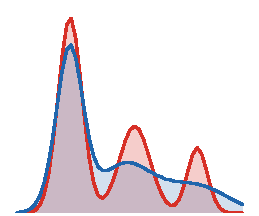
\includegraphics[width=.23\linewidth]{figures/martingale-ot-centered-kernels/marginals.pdf} &
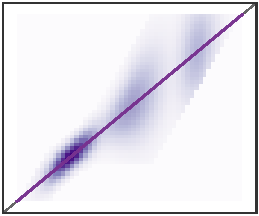
\includegraphics[width=.23\linewidth]{figures/martingale-ot-centered-kernels/generated-coupling.pdf} &
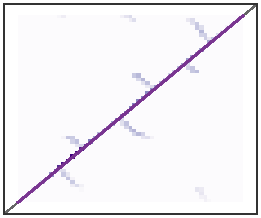
\includegraphics[width=.23\linewidth]{figures/martingale-ot-centered-kernels/optimal-coupling.pdf} &
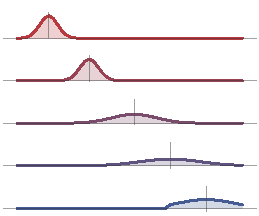
\includegraphics[width=.23\linewidth]{figures/martingale-ot-centered-kernels/conditionals.pdf}
\\[-.1em]
\small marginals & \small generated plan & \small optimal plan & \small centered kernels
\end{tabular}
\caption{\emph{A discrete one-dimensional martingale OT example.} The source $\alpha$ is a red Gaussian mixture on a grid. A first feasible plan is generated by centered kernels $K_i(y_j)=\kappa_i(y_j-x_i)$, whose discrete barycenter is $x_i$, so $P_{ij}=a_iK_i(y_j)$ satisfies $\bar T_P(x_i)=x_i$. Keeping the same two marginals, the third panel solves the finite-dimensional martingale OT linear program with objective $\sum_{ij}|x_i-y_j|P_{ij}$, row and column constraints, and martingale constraints $\sum_j(y_j-x_i)P_{ij}=0$. The optimized plan is much sparser, while both plans have the identity barycentric projection.}
\index{martingale OT}% strictindex
\index{convex!order}% strictindex
\index{barycentric!projection}% strictindex
\label{fig:martingale-ot-centered-kernels}
\end{figure}
